\chapter{LLM Cheat Sheet}

\section{Handling Imports from Parent Folders in Python and Jupyter}

When a Python script or Jupyter Notebook is located in a subfolder, modules in a parent folder may not be automatically discoverable by Python. The following methods illustrate how to properly import them.

\subsection{Using \_\_file\_\_ in Python Scripts}

For scripts executed directly, \_\_file\_\_ contains the path of the script. Use it to construct the parent folder path:

\begin{tcolorbox}[colback=red!5,colframe=red!70!black,title=Python Script: Using \_\_file\_\_]
\begin{verbatim}
import sys
import os

# Add parent folder to Python path
sys.path.append(os.path.abspath(os.path.join(os.path.dirname(__file__), '..')))

# Import module from parent folder
from LLMengineering import key_utils
\end{verbatim}
\end{tcolorbox}

\textbf{Explanation:}
\begin{itemize}
    \item \texttt{os.path.dirname(\_\_file\_\_)}: folder of the current script.
    \item \texttt{os.path.join(..., '..')}: go one level up.
    \item \texttt{os.path.abspath(...)}: get absolute path.
    \item \texttt{sys.path.append(...)}: add this path to Python's module search paths.
\end{itemize}

\subsubsection{Using \texttt{os.getcwd()} in Jupyter Notebooks}

In Jupyter, \_\_file\_\_ is not defined. Use the current working directory instead:

\begin{tcolorbox}[colback=gray!5, colframe=gray!80!black, title=Jupyter Notebook: Using os.getcwd()]
\begin{verbatim}
import sys
import os

# Add parent folder of current working directory
sys.path.append(os.path.abspath(os.path.join(os.getcwd(), '..')))

# Import module from parent folder
from key_utils import some_function
\end{verbatim}
\end{tcolorbox}

\textbf{Notes:}
\begin{itemize}
    \item \texttt{os.getcwd()}: returns the current working directory of the notebook.
    \item \texttt{..} moves one level up; \texttt{../..} moves two levels up.
    \item This approach is portable for notebooks without relying on \_\_file\_\_.
\end{itemize}

\subsubsection{Using Absolute Paths (Less Portable)}

\begin{tcolorbox}[colback=gray!5, colframe=gray!80!black, title=Absolute Path Approach]
\begin{verbatim}
import sys
sys.path.append("/run/media/sijanpaudel/New Volume/New folder/LLMengineering")

from key_utils import some_function
\end{verbatim}
\end{tcolorbox}


\textbf{Caution:} This works immediately but is hard-coded. If the project moves, the path must be updated.

\subsubsection{Recommended Long-Term Approach}

1. Add an empty \_\_init\_\_.py file in the parent folder (e.g., \texttt{LLMengineering/}) to make it a package.
2. Use relative or absolute imports within scripts:

\begin{tcolorbox}[colback=gray!5, colframe=gray!80!black, title=Long-Term Package Approach]
    \begin{verbatim}
    from LLMengineering import key_utils
    \end{verbatim}
\end{tcolorbox}

This makes imports clean, portable, and avoids repeated \texttt{sys.path.append} hacks.



\newpage
\section{Comparing LLMs -- The Basics (1)}
\begin{tabularx}{\textwidth}{|>{\hsize=0.3\hsize}L|>{\hsize=0.7\hsize}L|}
\hline
\textbf{Feature} & \textbf{Description / Notes} \\
\hline
Open-source or Closed & Whether the model’s weights, architecture, and training code are publicly available. Examples: GPT-4 (closed), LLaMA 2 (open). \\
\hline
Release Date \& Knowledge Cut-off & The date the model was released and the latest point in time the training data covers. Important for up-to-date responses. \\
\hline
Parameters & Number of trainable weights in the model (e.g., billions of parameters). Determines model capacity. \\
\hline
Training Tokens & Amount of text data used during training, usually in billions of tokens. More tokens generally improve performance. \\
\hline
Context Length & Maximum input length (in tokens) the model can handle in a single prompt. Longer context allows better understanding of large inputs. \\
\hline
\end{tabularx}

\vspace{1em}

\section{Comparing LLMs -- The Basics (2)}

\begin{tabularx}{\textwidth}{|>{\hsize=0.3\hsize}L|>{\hsize=0.7\hsize}L|}
\hline
\textbf{Feature} & \textbf{Description / Notes} \\
\hline
Inference Cost & Computational resources required to generate output (GPU, CPU usage). \\
\hline
API Charge / Subscription / Runtime Compute & How much it costs to access the model through a cloud service. \\
\hline
Training Cost & Cost to pretrain the model, including compute, electricity, and infrastructure. \\
\hline
Build Cost & Cost to fine-tune, deploy, or customize the model. \\
\hline
Time to Market & How quickly you can deploy and use the model in production. \\
\hline
Rate Limits & Restrictions on API usage, e.g., calls per minute or per day. \\
\hline
Speed \& Latency & How fast the model responds, depends on model size, hardware, and context length. \\
\hline
License & Terms for use, redistribution, and commercial deployment. Some open-source licenses restrict commercial use. \\
\hline
\end{tabularx}

\vspace{1em}

\section{Chinchilla Scaling Law}

\textbf{Key Principle:} Number of model parameters should scale roughly proportional to the number of training tokens.

\textbf{Implications:}
\begin{itemize}
    \item Increasing model size without enough data leads to plateaued or degraded performance.
    \item Having lots of training data with a small model underperforms; parameters must scale up.
\end{itemize}

\textbf{Rule of Thumb:} Let $N$ = model parameters, $D$ = training tokens. For optimal training:
\[
N \propto D
\]

\textbf{Example:}
\begin{itemize}
    \item Doubling model parameters $\rightarrow$ need roughly double the training tokens.
    \item Insufficient tokens $\rightarrow$ diminishing returns.
\end{itemize}

\textbf{Additional Notes:}
\begin{itemize}
    \item Smaller, well-trained models can outperform larger, undertrained ones.
    \item Helps determine compute-efficient configurations for new LLMs.
\end{itemize}

\vspace{1em}

\section{Common LLM Benchmarks}
\begin{tabularx}{\textwidth}{|>{\hsize=0.2\hsize}X|>{\hsize=0.3\hsize}X|>{\hsize=0.5\hsize}X|}
\hline
\textbf{Benchmark} & \textbf{Focus / Task} & \textbf{Description} \\
\hline
MMLU & Knowledge across multiple subjects & Assess general knowledge and reasoning; used to compare models like GPT-3, Chinchilla, and Gopher. \\
\hline
BIG-bench & Broad suite of diverse reasoning tasks & Tests reasoning, factual knowledge, ethics, math, code; hundreds of tasks evaluating beyond narrow QA. \\
\hline
HellaSwag & Commonsense reasoning & Multiple-choice questions for everyday situations; measures ability to predict plausible outcomes. \\
\hline
TruthfulQA & Factual accuracy / truthfulness & QA tasks designed to detect hallucinations; evaluates honesty of LLM answers. \\
\hline
WinoGrande / Winograd Schema Challenge & Pronoun resolution / coreference & Tests commonsense reasoning and context understanding; resolves ambiguous references. \\
\hline
ARC & Science and reasoning & Multiple-choice science questions; evaluates problem-solving and reasoning in STEM. \\
\hline
HumanEval & Coding and code generation & Tests Python programming ability; measures functional correctness of generated code. \\
\hline
\end{tabularx}

\vspace{1em}

\section{Specific Benchmarks}

\begin{tabularx}{\textwidth}{|>{\hsize=0.2\hsize}X|>{\hsize=0.3\hsize}X|>{\hsize=0.5\hsize}X|}
\hline
\textbf{Benchmark} & \textbf{What’s Being Evaluated} & \textbf{Description} \\
\hline
ELO & Model ranking / performance consistency & Evaluates models via pairwise comparisons; creates a relative ranking of LLMs across multiple tasks. \\
\hline
HumanEval & Code generation / functional correctness & Tests an LLM’s ability to write Python functions that pass unit tests; measures coding logic and correctness. \\
\hline
Multipl-E & Multimodal reasoning & Evaluates LLMs on tasks combining text and images (or multiple modalities); measures reasoning and comprehension across modalities. \\
\hline
\end{tabularx}

\vspace{1em}

\section{Limitations of Benchmarks}

\begin{tabularx}{\textwidth}{|>{\hsize=0.6\hsize}L|>{\hsize=1.4\hsize}L|}
\hline
\textbf{Limitation} & \textbf{Explanation} \\
\hline
Narrow focus & Many benchmarks test only specific skills (e.g., coding, factual QA, commonsense), not overall intelligence or adaptability. \\
\hline
Static datasets & Benchmarks are fixed in time, so models trained after the cut-off may have an unfair advantage or miss newer knowledge. \\
\hline
Lack of real-world context & Benchmarks often use idealized tasks, not messy, ambiguous, or multi-step real-world scenarios. \\
\hline
Gaming / overfitting & Models can be fine-tuned or prompted to specifically excel on benchmark tasks without improving general capabilities. \\
\hline
Limited multimodality & Most benchmarks focus on text-only tasks; few measure image, audio, or multimodal reasoning. \\
\hline
Subjectivity & Some benchmarks (e.g., ethics, creativity, hallucination detection) are hard to score objectively. \\
\hline
Compute bias & Larger models may perform better mainly due to size, not reasoning ability, skewing benchmark results. \\
\hline
Hard to measure nuanced reasoning & Benchmarks mostly measure surface correctness; they often cannot capture multi-step reasoning, context-dependent judgment, creativity, or reasoning accuracy vs. fluency. \\
\hline
\end{tabularx}

\section{Advanced Benchmarks for Large Language Models}

\begin{tabularx}{\textwidth}{|>{\hsize=0.2\hsize}X|>{\hsize=0.3\hsize}X|>{\hsize=0.5\hsize}X|}
\hline
\textbf{Benchmark} & \textbf{Focus / Task} & \textbf{Description / Meaning} \\
\hline
GPQA & Graduate-level question answering & Evaluates performance on graduate-level tests with 448 expert questions. Non-PhD humans score only 34\% even with web access. Measures LLM ability to handle highly specialized knowledge. \\
\hline
BBHard & Future capabilities & Includes 204 tasks previously thought beyond LLM capabilities. Designed to test reasoning, logic, and generalization at a next-level difficulty. \\
\hline
Math Lv 5 & High-school math competition problems & Measures model’s ability to solve advanced math problems requiring multi-step reasoning and problem-solving skills. Useful for chain-of-thought evaluation. \\
\hline
IFEval & Instruction following & Tests the model’s ability to follow complex instructions, e.g., “write more than 400 words” and “mention AI at least 3 times.” Evaluates comprehension and compliance with nuanced prompts. \\
\hline
MuSR & Multistep soft reasoning & Assesses logical deduction and multi-step reasoning. Example: analyzing a 1,000-word story and identifying “who has means, motive, and opportunity.” Tests reasoning beyond surface facts. \\
\hline
MMLU-PRO & Harder MMLU version & Advanced, cleaned-up version of MMLU with questions having 10 possible answers instead of 4. Evaluates deeper knowledge, multi-choice reasoning, and generalization. \\
\hline
\end{tabularx}

\vspace{1em}
\textbf{Notes:}
\begin{itemize}
    \item These benchmarks are considered “next-level” because they test advanced reasoning, multi-step logic, and high-level knowledge.  
    \item Useful for evaluating models that go beyond standard QA, commonsense reasoning, or basic coding tasks.  
    \item Many of these benchmarks also measure compliance with complex instructions and reasoning under uncertainty. 
\end{itemize}


\begin{tabularx}{\textwidth}{|>{\hsize=0.15\hsize}X|>{\hsize=0.85\hsize}X|}
\hline
\textbf{Benchmark} & \textbf{Purpose / Examples} \\
\hline
GPQA & Specialized knowledge, expert-level Q\&A, academic reasoning, physics, chemistry, biology expertise.  \newline
\textbf{Examples:} Explain the biochemical steps of glycolysis; Describe Newton’s laws with practical applications; Explain photosynthesis in detail. \\
\hline
BBHard & Advanced reasoning, logic, generalization in challenging scenarios.  \newline
\textbf{Examples:} Predict how a hypothetical AI agent could optimize a supply chain in a novel scenario; Design a strategy to minimize energy consumption in an unfamiliar industrial process; Solve a logic puzzle with multiple constraints. \\
\hline
Math Lv 5 & Complex problem solving, chain-of-thought evaluation, mathematical reasoning.  \newline
\textbf{Examples:} Solve: If \(x^2 - 5x + 6 = 0\), find all integer solutions; Evaluate combinatorial problems like “How many ways can 5 books be arranged on a shelf?”; Solve calculus problems requiring multiple steps. \\
\hline
IFEval & Precise instruction compliance, comprehension, content generation with constraints.  \newline
\textbf{Examples:} Write a 450-word essay on renewable energy mentioning AI at least 3 times; Summarize a research paper in 300 words including key terms; Rewrite a paragraph to follow a formal tone while keeping original meaning. \\
\hline
MuSR & Multi-step reasoning, deduction, understanding narratives beyond surface facts, solving prime puzzles and reasoning tasks.  \newline
\textbf{Examples:} Analyze a 1,000-word mystery story to determine “who has means, motive, and opportunity”; Identify the next prime number in a complex sequence; Solve multi-step logic puzzles. \\
\hline
MMLU-PRO & Deep knowledge, advanced multi-choice understanding, broader knowledge evaluation, general language understanding.  \newline
\textbf{Examples:} Choose the best explanation for why the sky is blue from 10 options; Identify the correct historical fact among 10 alternatives; Evaluate grammar and style in multiple-choice questions. \\
\hline
\end{tabularx}

\vspace{0.5em}
\textbf{Tips to distinguish benchmarks:}
\begin{itemize}
    \item \textbf{GPQA} -- focus on subject expertise.
    \item \textbf{BBHard} -- focus on novel reasoning and logic.
    \item \textbf{IFEval} -- focus on following instructions accurately.
    \item \textbf{MuSR} -- focus on multi-step deduction and problem solving (e.g., prime puzzles, mysteries).
    \item \textbf{MMLU-PRO} -- focus on broad knowledge and multiple-choice reasoning.
\end{itemize}


\section{Leaderboard Image}

% Include the image
\begin{center}
\includegraphics[width=0.8\textwidth]{leaderboards.png}
\end{center}

\begin{tabularx}{\textwidth}{|>{\hsize=0.6\hsize}L|>{\hsize=1.4\hsize}L|}
\hline
\textbf{Leaderboard} & \textbf{Purpose / Use} \\
\hline
HuggingFace Open LLM & Tracks performance of open-source LLMs (new and old versions). Useful for selecting models for research or deployment with full weight access. \\
\hline
HuggingFace BigCode & Focused on code generation LLMs. Helps compare models for coding tasks, programming language coverage, and code quality. \\
\hline
HuggingFace LLM Perf & Benchmarking general LLM performance across various NLP tasks. Useful for measuring speed, accuracy, RAM memory usage and general reasoning ability. \\
\hline
HuggingFace Others & Specialized leaderboards, e.g., medical, domain-specific, or language-specific models. Guides selection for niche applications. \\
\hline
Vellum & Includes context window, API cost, and usage constraints. Useful for developers to choose models based on practical deployment factors. \\
\hline
SEAL & Focused on expert skills and high-level reasoning. Useful for selecting LLMs that excel in professional or complex knowledge domains. \\
\hline
\end{tabularx}

\newpage
\section{A 5-Step Strategy for Using AI Models}
This is a simple guide to choosing, training, and using a Large Language Model (LLM) to solve a real-world business problem.
\begin{center}
\includegraphics[width=1\textwidth]{strategy.png}
\end{center}


\newpage
\subsection{Understand (Figure Out What You Need)}
Before you start, you need a clear plan. Think about what you're trying to achieve.

\begin{itemize}
    \item \textbf{Gather Business Needs:} What is the specific problem you want the AI to solve? (e.g., "Answer customer support questions automatically.")
    \item \textbf{Define Success:} How will you know if the AI is doing a good job? Focus on what matters to the business, not just technical scores. (e.g., "Reduce customer wait times by 50%.")
    \item \textbf{Look at Your Data:} What information do you have? Is it a lot? Is it messy or clean? What format is it in?
    \item \textbf{Consider the Limits:} Think about the practical stuff.
    \begin{itemize}
        \item How much money can you spend?
        \item Does it need to be super fast?
        \item How many people will be using it?
        \item What is the deadline to get this working?
    \end{itemize}
\end{itemize}

% Include the image
\begin{center}
\includegraphics[width=1\textwidth]{understand.png}
\end{center}

\newpage
\subsection{Prepare (Do Your Homework)}
Once you have a plan, it's time to get your resources ready.

\begin{itemize}
    \item \textbf{Research Solutions:} See how this problem is already being solved. Look at solutions that don't use a big AI model to set a "baseline" for performance.
    \item \textbf{Compare AI Models:} Look at different LLMs.
    \begin{itemize}
        \item \textbf{The Basics:} How much do they cost? How much text can they handle at once (context length)? Can you legally use them for your business?
        \item \textbf{Performance:} Check online tests (Benchmarks, Leaderboards) to see which models are best at certain tasks.
    \end{itemize}
    \item \textbf{Clean Your Data:} This is very important! You need to organize, clean, and prepare your data so the AI can learn from it effectively.
\end{itemize}
\begin{center}
\includegraphics[width=1\textwidth]{prepare.png}
\end{center}

\newpage
\subsection{Select (Pick Your Tools and Test Them)}
Now you can choose your model and see how it performs with your data.

\begin{itemize}
    \item \textbf{Choose Your LLM(s):} Based on your research, pick one or two models that seem like the best fit.
    \item \textbf{Experiment:} Play around with the models. See what they're good at and where they struggle.
    \item \textbf{Train and Check:} Use your clean data to test (validate) the models to get real performance numbers.
\end{itemize}
\begin{center}
\includegraphics[width=1\textwidth]{select.png}
\end{center}
\newpage
\subsection{Customize (Make the AI Better at Your Task)}
Out-of-the-box models are good, but you can make them great by using special techniques to improve their performance on your specific problem. There are three main ways to do this.

\subsubsection{Three Key Techniques}

\begin{description}
    \item[Prompting] \hfill \\
    This means giving the AI better instructions. It's the fastest and cheapest way to improve performance. You can give it examples, tell it to "think step-by-step," or connect it to other software tools.
    \item[RAG (Retrieval-Augmented Generation)] \hfill \\
    This is like giving the AI an "open book" for a test. You connect the model to a knowledge base (like your company's internal documents). When a question is asked, the AI first finds the relevant information from your documents and then uses that information to create the answer. This ensures the answers are accurate and up-to-date.
    \item[Fine-Tuning] \hfill \\
    This is the most advanced technique. You actually re-train a part of the AI model on your own data. This teaches the model a new skill or a specific style, making it an expert in your particular area. It's expensive and requires a lot of data but can lead to the best performance.
\end{description}
\begin{center}
\includegraphics[width=1\textwidth]{Customize.png}
\end{center}
\newpage
\subsubsection{Comparing the Three Techniques}

\begin{tcolorbox}[title=Pros: The Good Stuff, boxrule=1pt, sharp corners]
\begin{tabular}{p{0.3\linewidth} | p{0.3\linewidth} | p{0.3\linewidth}}
    \textbf{Prompting} & \textbf{RAG} & \textbf{Fine-tuning} \\
    \hline
    1. Quick to do & 1. More accurate answers & 1. Creates a true expert \\
    2. Cheap & 2. Works with lots of data & 2. Understands subtle details \\
    3. See improvements right away & 3. Efficient & 3. Can learn a specific tone or style \\
     &  & 4. Faster and cheaper answers \\
\end{tabular}
\end{tcolorbox}

\begin{tcolorbox}[title=Cons: The Downsides, boxrule=1pt, sharp corners]
\begin{tabular}{p{0.3\linewidth} | p{0.3\linewidth} | p{0.3\linewidth}}
    \textbf{Prompting} & \textbf{RAG} & \textbf{Fine-tuning} \\
    \hline
    1. Limited by how much text the AI can read at once & 1. More complex to set up & 1. Takes a lot of effort \\
    2. Improvements eventually stop & 2. Needs accurate, up-to-date info & 2. Needs a lot of clean data \\
    3. Can be slow and expensive for each answer & 3. Can miss subtle details & 3. Costs money to train \\
     &  & 4. Risk of the AI forgetting its original general knowledge \\
\end{tabular}
\end{tcolorbox}

\begin{center}
\includegraphics[width=1\textwidth]{pros.png}
\end{center}


\begin{center}
\includegraphics[width=1\textwidth]{cons.png}
\end{center}


\begin{center}
\includegraphics[width=1\textwidth]{usecases.png}
\end{center}

\newpage
\subsection{Productionize (Get It Ready for the Real World)}
Once the model is working well, you need to make it a reliable part of your business.

\begin{itemize}
    \item \textbf{Connect it:} How will your website or other software "talk" to the AI model?
    \item \textbf{Deploy it:} Where will the model run? On your own computers or in the cloud?
    \item \textbf{Plan for Growth:} What happens if you get thousands of users? Make sure it's secure, and you're monitoring it for problems.
    \item \textbf{Measure What Matters:} Go back to Step 1 and measure the business goals you set. Is it actually working?
    \item \textbf{Keep it Updated:} Continuously check the AI's performance and re-train it with new data to keep it from becoming outdated.
\end{itemize}


\begin{center}
\includegraphics[width=1\textwidth]{productionize.png}
\end{center}
\begin{center}
\includegraphics[width=1\textwidth]{traditional.png}
\end{center}

\newpage
\section{LoRA (Low-Rank Adaptation)}

\subsection{Introduction}
LoRA (Low-Rank Adaptation) is a technique designed to \textbf{fine-tune large pre-trained models efficiently}. Large language models (LLMs) like GPT, LLaMA, etc., have \textbf{billions of parameters}, making traditional fine-tuning:

\begin{itemize}
    \item Extremely expensive in computation.
    \item Memory-intensive.
    \item Hard to maintain multiple fine-tuned versions.
\end{itemize}

LoRA solves this by training \textbf{small, additional modules} instead of updating the entire model.

\subsubsection{How LoRA Works (Detailed)}
Consider a weight matrix in a neural network layer:  
\[
W \in \mathbb{R}^{d \times k}
\]
Full fine-tuning adjusts every element in $W$, which is costly.  

LoRA introduces \textbf{two low-rank matrices} $A$ and $B$ and approximates the weight update:
\[
\Delta W \approx A B
\]
where:
\[
A \in \mathbb{R}^{d \times r}, \quad B \in \mathbb{R}^{r \times k}, \quad r \ll \min(d, k)
\]

Key points:  
\begin{itemize}
    \item $r$ is small, so $A$ and $B$ are \textbf{tiny compared to $W$}.
    \item Only $A$ and $B$ are trained; the original $W$ is \textbf{frozen}.
    \item Memory and computation are drastically reduced.
\end{itemize}

\subsubsection{Step-by-Step Intuition}
\begin{enumerate}
    \item Start with a pre-trained model whose parameters $W$ are \textbf{frozen}.
    \item Add small trainable matrices $A$ and $B$ to selected layers (often attention layers).
    \item Forward pass: compute original output using $W$ and add low-rank contribution:  
    \[
    y = W x + \alpha (A B x)
    \]
    where $\alpha$ is a scaling factor.
    \item Backpropagation only updates $A$ and $B$, leaving $W$ untouched.
    \item After training, save only $A$ and $B$ as the \textbf{LoRA adapter}.
\end{enumerate}

\subsubsection{Simple Analogy}
\begin{tcolorbox}[colback=green!5!white,colframe=green!75!black,title=Analogy]
Think of a professional camera with many settings:

\begin{itemize}
    \item Full fine-tuning = manually adjusting every knob and lens component each time you want a new photo style.
    \item LoRA = keep the camera fixed, but attach a \textbf{small filter}. 
\end{itemize}

The filter is light, cheap, and can be swapped out, while the main camera stays unchanged.
\end{tcolorbox}

\subsubsection{Why LoRA is Effective}
\begin{itemize}
    \item Neural network updates often lie in a \textbf{low-rank subspace}, so approximating with small matrices captures most of the needed changes.
    \item Reduces training cost dramatically.
    \item Reduces storage: instead of storing full fine-tuned model (~10s of GB), store just adapters (~10s of MB).
    \item Enables \textbf{multi-tasking}: use same base model with different adapters for different tasks.
\end{itemize}

\subsubsection{Benefits vs Limitations}
\begin{tcolorbox}[colback=blue!5!white,colframe=blue!75!black,title=Pros]
\begin{itemize}
    \item \textbf{Memory-efficient} and fast training.
    \item Base model remains \textbf{unchanged}, enabling multiple adapters.
    \item Easy integration with pre-trained models.
\end{itemize}
\end{tcolorbox}

\begin{tcolorbox}[colback=red!5!white,colframe=red!75!black,title=Cons]
\begin{itemize}
    \item Only works well when \textbf{low-rank approximation is sufficient}.
    \item Might not capture highly complex changes needed for very different tasks.
\end{itemize}
\end{tcolorbox}

\subsubsection{Summary in Simple Words}
\begin{tcolorbox}[colback=blue!5!white,colframe=blue!75!black,title=LoRA Simplified]
You can think of LoRA as adding \textbf{tiny adapters on top of a frozen large model}.  

Imagine a giant model with billions of knobs. Fine-tuning everything is slow and expensive.  

LoRA adds a few small sliders (matrices) on top of the frozen model.  
During training, only these sliders move, but they are enough to guide the model to a new task.
\end{tcolorbox}
\newpage
\subsubsection{Visualization Idea}
You can include a visual showing LoRA adapters on top of a frozen model:
\href{https://blog.dailydoseofds.com/p/full-model-fine-tuning-vs-lora-vs}{Link}



\href{https://substackcdn.com/image/fetch/$s_!igxz!,f_auto,q_auto:good,fl_progressive:steep/https%3A%2F%2Fsubstack-post-media.s3.amazonaws.com%2Fpublic%2Fimages%2F1b402882-3dc1-4d5b-ba11-7f4f6d40d888_914x1116.gif}{%
    \includegraphics[width=1\textwidth]{lora.png}%
}
\newpage
\section{LoRA Hyperparameters: $r$, $\alpha$, and Target Modules}

LoRA (Low-Rank Adaptation) introduces a few crucial hyperparameters that control the learning capacity, scaling, and location of the adaptation. Understanding them is key to effective fine-tuning.

\subsection{Rank $r$ (Low-Rank Dimension)}
The hyperparameter $r$ determines the \textbf{rank of the low-rank matrices} $A \in \mathbb{R}^{d \times r}$ and $B \in \mathbb{R}^{r \times k}$.  

\begin{itemize}
    \item Controls the number of parameters introduced in the LoRA adapter.
    \item Small $r$ $\Rightarrow$ fewer parameters, less memory, faster training, but less expressive.
    \item Large $r$ $\Rightarrow$ more parameters, higher capacity, but increased memory and computation.
\end{itemize}

\textbf{Rule of Thumb:}  
\begin{tcolorbox}[colback=blue!5!white,colframe=blue!75!black]
Start with $r \in [4, 64]$ for LLMs. Increase $r$ if the task is complex or performance is insufficient.
\end{tcolorbox}

\subsubsection{Scaling Factor $\alpha$}
The hyperparameter $\alpha$ scales the output of the LoRA adapter:

\[
y = W x + \frac{\alpha}{r} (A B x)
\]

\begin{itemize}
    \item Controls the \textbf{strength of the low-rank update} relative to the original weights.
    \item Small $\alpha$ $\Rightarrow$ subtle influence, safer but slower adaptation.
    \item Large $\alpha$ $\Rightarrow$ strong influence, faster adaptation, but may destabilize training.
\end{itemize}

\textbf{Rule of Thumb:}  
\begin{tcolorbox}[colback=green!5!white,colframe=green!75!black]
Use $\alpha \in [8, 32]$ for LLMs. Adjust based on task difficulty and stability.
\end{tcolorbox}

\subsubsection{Target Modules}
Target modules define \textbf{which layers of the base model receive LoRA adapters}.  

\begin{itemize}
    \item Common targets: attention layers (query/key/value), feed-forward layers.  
    \item Choosing too many modules $\Rightarrow$ more parameters, higher memory.  
    \item Choosing too few modules $\Rightarrow$ may underfit the task.
\end{itemize}

\textbf{Rule of Thumb:}  
\begin{tcolorbox}[colback=yellow!5!white,colframe=yellow!75!black]
Start by adding LoRA to attention projection matrices (query and value) for LLMs. Expand to feed-forward layers only if necessary.
\end{tcolorbox}

\subsection{Summary Table}

\begin{tcolorbox}[colback=gray!5!white,colframe=black,title=LoRA Hyperparameters Summary]
\begin{tabular}{|p{4cm}|p{5cm}|p{6cm}|}
\hline
\textbf{Hyperparameter} & \textbf{Role} & \textbf{Rule of Thumb} \\
\hline
$r$ & Low-rank dimension (number of adapter parameters) & 4--64 \\
\hline
$\alpha$ & Scaling factor of LoRA update & 8--32 \\
\hline
Target Modules & Layers where adapters are applied & Start with attention layers and then expand to feed-forward layers only if necessary. \\
\hline
\end{tabular}
\end{tcolorbox}


\includegraphics[width=1\textwidth]{parameter.png}
\newpage
\section{Q, K, V, O in Transformers}

In a transformer model, the attention mechanism allows each token to selectively focus on other tokens in the sequence. This is done using four key components: \textbf{Query (Q)}, \textbf{Key (K)}, \textbf{Value (V)}, and \textbf{Output (O)}.  

\begin{itemize}
    \item \textbf{Query (Q):} Represents the \textbf{questions} each token asks. For example, a token may ask, ``Which other tokens are relevant to me?'' Q is calculated by multiplying the token embedding with a learned weight matrix $W_Q$.
    
    \item \textbf{Key (K):} Represents the \textbf{tags or identifiers} of each token. It helps the Query figure out which tokens are relevant. K is computed by multiplying token embeddings with another learned weight matrix $W_K$.
    
    \item \textbf{Value (V):} Represents the \textbf{actual content or information} of each token. Once Q identifies which tokens are relevant (by comparing with K), V provides the information to pass forward. V is calculated using the weight matrix $W_V$.
    
    \item \textbf{Output (O):} After attention combines relevant V vectors, O is a projection that mixes the attended information back into the model’s hidden dimension using the matrix $W_O$. This ensures the output can be passed to the next layer seamlessly.
\end{itemize}

The attention operation is mathematically defined as:

\[
\text{Attention}(Q,K,V) = \text{softmax}\Big(\frac{QK^\top}{\sqrt{d_k}}\Big)V
\]

\begin{itemize}
    \item $QK^\top$ computes the similarity between queries and keys.  
    \item $d_k$ is the \textbf{dimension of the key vectors per attention head}. Dividing by $\sqrt{d_k}$ scales the dot product so that the softmax does not produce extremely small or large probabilities.  
    \item Multiplying by $V$ gathers the relevant information based on these attention weights.
\end{itemize}

\subsection{Analogy: Classroom Example}

\begin{tcolorbox}[colback=yellow!5!white,colframe=yellow!75!black,title=Analogy]
Imagine a classroom scenario where students ask and answer questions:

\begin{itemize}
    \item \textbf{Q (Query):} A student asks a question to figure out which other students have relevant information.
    \item \textbf{K (Key):} Each student has a topic card that indicates what they know.
    \item \textbf{V (Value):} Each student provides an answer (information) if their topic matches the query.
    \item \textbf{O (Output):} The teacher collects all answers, summarizes them, and writes a combined response on the board.
    \item \textbf{$d_k$:} Think of it as the “attention focus resolution” — how detailed each student’s topic card is. More details (larger $d_k$) require scaling to prevent overemphasis on any single answer.
\end{itemize}

This shows how Q identifies what to focus on, K helps determine relevance, V provides the information, and O produces the final output.
\end{tcolorbox}


\newpage
\section{LoRA in PeftModelForCausalLM}


\subsection{Model Architecture Overview}

The \texttt{PeftModelForCausalLM} wraps a \texttt{LlamaForCausalLM} base model and applies \textbf{LoRA adapters} for efficient fine-tuning.

\begin{itemize}
    \item \textbf{Embedding Layer:} \texttt{embed\_tokens} maps vocabulary tokens (128256) to embeddings of size 4096.
    \item \textbf{Decoder Layers:} 32 \texttt{LlamaDecoderLayer} modules, each containing:
        \begin{itemize}
            \item \textbf{Self-Attention (\texttt{self\_attn})}
                \begin{itemize}
                    \item Q, K, V, O projections use \texttt{lora.Linear4bit} modules.
                    \item Each projection has:
                        \begin{itemize}
                            \item \texttt{base\_layer}: The frozen 4-bit linear layer representing the main weight matrix.
                            \item \texttt{lora\_A}, \texttt{lora\_B}: Low-rank matrices (rank $r=32$) representing trainable updates.
                            \item \texttt{lora\_dropout}: Dropout for regularization.
                        \end{itemize}
                    \item LoRA modifies only the projection weights, not the base model.
                \end{itemize}
            \item \textbf{Feed-Forward Network (MLP):} \texttt{LlamaMLP} with:
                \begin{itemize}
                    \item \texttt{gate\_proj} and \texttt{up\_proj} (expand embeddings to 14336)  
                    \item \texttt{down\_proj} (reduce back to 4096)  
                    \item Non-linearity: \texttt{SiLU()}
                \end{itemize}
            \item \textbf{LayerNorms:} \texttt{input\_layernorm} and \texttt{post\_attention\_layernorm}.
            \item \textbf{Rotary Positional Embeddings:} \texttt{rotary\_emb} for relative position encoding.
        \end{itemize}
    \item \textbf{Final LayerNorm:} \texttt{norm} over the hidden dimension.
    \item \textbf{LM Head:} Linear mapping from hidden size 4096 to vocabulary size 128256.
\end{itemize}

\subsection{LoRA in Attention Layers}

In transformers, attention is computed as:

\[
\text{Attention}(Q,K,V) = \text{softmax}\Big(\frac{Q K^\top}{\sqrt{d_k}}\Big) V
\]

where Q, K, V are projections of the input embeddings. LoRA modifies these projections as follows:

\[
W_{\text{proj}} \rightarrow W_{\text{proj}} + \Delta W = W_{\text{proj}} + A B
\]

\begin{itemize}
    \item $W_{\text{proj}}$ is the frozen base projection weight (Linear4bit).
    \item $A \in \mathbb{R}^{d_{\text{model}} \times r}$, $B \in \mathbb{R}^{r \times d_{\text{proj}}}$, with $r \ll d_{\text{model}}$ (e.g., $r=32$).  
    \item Only $A$ and $B$ are trainable, drastically reducing the number of parameters.
    \item LoRA is applied individually to \textbf{Q, K, V, O} matrices:
        \begin{itemize}
            \item \texttt{q\_proj}: 4096 $\rightarrow$ 4096
            \item \texttt{k\_proj}: 4096 $\rightarrow$ 1024
            \item \texttt{v\_proj}: 4096 $\rightarrow$ 1024
            \item \texttt{o\_proj}: 4096 $\rightarrow$ 4096
        \end{itemize}
\end{itemize}

\subsubsection{Why LoRA is Effective in Attention}

\begin{itemize}
    \item \textbf{Memory Efficiency:} Instead of updating the full weight matrices (4096$\times$4096), only two small matrices of size 4096$\times$32 and 32$\times$4096 are trained per projection.
    \item \textbf{Task Adaptation:} LoRA can inject task-specific knowledge into the attention mechanism without modifying the base model.
    \item \textbf{Multiple Adapters:} Different LoRA adapters can be swapped for different tasks while keeping the same base model frozen.
    \item \textbf{Attention-Focused Learning:} By applying LoRA specifically to Q, K, V, O, the model learns to adjust how it attends to other tokens, which is sufficient for most fine-tuning tasks.
\end{itemize}

\subsection{Dimensions of Q, K, V, O Projections}

\begin{tcolorbox}[colback=blue!5!white,colframe=blue!75!black,title=Attention Projection Dimensions]
\begin{tabular}{|c|c|c|}
\hline
\textbf{Projection} & \textbf{Input Features} & \textbf{Output Features} \\
\hline
Q (\texttt{q\_proj}) & 4096 & 4096 \\
K (\texttt{k\_proj}) & 4096 & 1024 \\
V (\texttt{v\_proj}) & 4096 & 1024 \\
O (\texttt{o\_proj}) & 4096 & 4096 \\
\hline
\end{tabular}
\end{tcolorbox}

\subsection{Summary}

\begin{itemize}
    \item \textbf{LoRA} allows fine-tuning of very large models with minimal additional parameters.  
    \item Applied to attention layers, LoRA adjusts how the model attends to input tokens.  
    \item Memory-efficient and task-adaptive: only the low-rank matrices are trained, while the main model stays frozen.  
    \item Facilitates multiple task-specific adapters without retraining the entire model.
\end{itemize}

\subsubsection{Key Points}

\begin{itemize}
    \item $d_{\text{model}}$ is the hidden dimension (4096 in this model) through which all tokens are projected.
    \item LoRA adds small trainable matrices (rank $r = 32$) to Q, K, V, O projections.
    \item Base projections remain frozen; only adapters are updated.
    \item Memory-efficient and task-adaptive fine-tuning.
\end{itemize}

\newpage
\section{Loading a Base Model in 4-Bit and Using LoRA}

The following code demonstrates how to load a large language model (LLM) in 4-bit precision for memory efficiency and later fine-tune it with LoRA.

\begin{verbatim}
quant_config = BitsAndBytesConfig(
    load_in_4bit=True,
    bnb_4bit_use_double_quant=True,
    bnb_4bit_compute_dtype=torch.bfloat16,
    bnb_4bit_quant_type="nf4")

base_model = AutoModelForCausalLM.from_pretrained(
    BASE_MODEL,
    quantization_config=quant_config,
    device_map="auto",
)
\end{verbatim}

\subsection{Explanation of the Code}

\begin{itemize}
    \item \textbf{BitsAndBytesConfig}: Configuration for quantization. Quantization reduces the precision of the weights to save memory.
    \begin{itemize}
        \item \texttt{load\_in\_4bit=True}: Load model weights in 4-bit precision instead of 16-bit or 32-bit, drastically reducing memory usage.
        \item \texttt{bnb\_4bit\_use\_double\_quant=True}: Uses double quantization to reduce numerical errors and improve accuracy.
        \item \texttt{bnb\_4bit\_compute\_dtype=torch.bfloat16}: Performs computations in bfloat16 to maintain performance while saving memory.
        \item \texttt{bnb\_4bit\_quant\_type="nf4"}: Specifies the 4-bit quantization type.
    \end{itemize}
    
    \item \textbf{AutoModelForCausalLM.from\_pretrained}: Loads the pre-trained LLM with the above quantization configuration.
    \begin{itemize}
        \item \texttt{BASE\_MODEL}: The pre-trained model identifier (e.g., LLaMA, Falcon).
        \item \texttt{quantization\_config=quant\_config}: Uses the 4-bit quantized weights for memory efficiency.
        \item \texttt{device\_map="auto"}: Automatically maps model layers to available GPU(s) or CPU.
    \end{itemize}
\end{itemize}

\subsection{How LoRA Optimizes This}

\begin{itemize}
    \item Loading the model in 4-bit reduces the memory footprint, but full fine-tuning is still expensive if we try to update all weights.
    \item LoRA introduces \textbf{small trainable adapters} (low-rank matrices $A$ and $B$) on top of the frozen base model.
    \item Only these adapters are updated during training, allowing:
    \begin{itemize}
        \item \textbf{Memory efficiency}: base model weights are frozen and quantized.
        \item \textbf{Faster training}: fewer parameters are trained.
        \item \textbf{Task adaptation}: the model can specialize on a new task without full fine-tuning.
    \end{itemize}
    \item Effectively, combining 4-bit quantization with LoRA allows training huge models on limited GPU memory.
\end{itemize}

\subsection{Summary}

\begin{tcolorbox}[colback=blue!5!white,colframe=blue!75!black,title=Takeaway]
\begin{itemize}
    \item \textbf{4-bit quantization}: reduces memory usage of base model weights.
    \item \textbf{LoRA adapters}: trainable low-rank matrices that update model behavior without touching the large frozen base model.
    \item \textbf{Combined benefit}: efficient fine-tuning on large models with low GPU memory and compute cost.
\end{itemize}
\end{tcolorbox}

\newpage

\section{Decision: Selecting a Base Model}

\subsection{Goal}
Choose a base model by balancing: \textbf{task requirements}, \textbf{inference cost (latency / GPU memory)}, \textbf{accuracy needs}, \textbf{license / ecosystem}, and \textbf{how you plan to fine-tune (LoRA, RAG, full FT)}.

\subsection{Decision criteria (short checklist)}
\begin{itemize}
  \item \textbf{Capability vs cost:} larger models usually perform better but cost more to run and host.
  \item \textbf{Parameter count:} affects memory, quantization decisions and latency.
  \item \textbf{Context window / multimodality:} needed for long-context tasks or image+text.
  \item \textbf{License and ecosystem:} open weights, available tooling (HF, vendor SDKs), community adapters.
  \item \textbf{Fine-tuning strategy:} if you plan to use LoRA, favor models with stable adapter support and documented PEFT integrations.
  \item \textbf{Deployment target:} edge / mobile vs single-GPU vs multi-GPU / cloud inference.
\end{itemize}

\subsection{Model-by-model short summary}
\begin{itemize}
  \item \textbf{LLaMA family (Meta)}: a family of open/available models offered in multiple sizes (smaller local-friendly models and very large variants for research). LLaMA models are widely used for research and community tooling; instruction-tuned variants (``instruct'') are offered for easier instruction-following. 
  \item \textbf{Qwen (Alibaba)}: a rapidly-evolving family with strong claims in multilingual and code tasks; recent releases include much larger variants (cutting-edge, often multimodal and optimized for large-scale deployments).
  \item \textbf{Phi (Microsoft / Phi family)}: smaller, efficient models (e.g., Phi-2 at a few billion parameters) that are optimized for reasoning and cost-effective deployments at smaller parameter counts.
  \item \textbf{Gemma (Google / DeepMind family)}: a family of lightweight-to-mid-size models intended for efficient, practical use (good on-device and cloud tradeoffs); models come in small-to-medium sizes optimized for production usage.
\end{itemize}

\subsection{Comparison table (high-level)}
\begin{tcolorbox}[colback=gray!5!white,colframe=black,title=Model comparison at a glance]
\begin{tabular}{|p{2cm}|p{3cm}|p{4cm}|p{5.0cm}|}
\hline
\textbf{Model} & \textbf{Representative sizes} & \textbf{Typical strengths} & \textbf{Suggested use-cases / notes} \\
\hline
LLaMA (Meta) & 8B, 70B, (and larger research variants) & Strong general-purpose language and reasoning; broad community tooling & Good when you want high-quality open models and lots of community adapters; choose size by budget \\
\hline
Qwen (Alibaba) & Ranges from mid-size up to very large (vendor evolving family, latest pushes into extremely large sizes) & Good for code, multilingual tasks and large-scale deployments & Consider for enterprise cloud deployments or when vendor benchmarks favour Qwen for your task \\
\hline
Phi (Microsoft) & Small/medium (e.g., ~2.7B for Phi-2) & Very cost-efficient; strong small-model reasoning per-cost & Excellent for edge or low-cost cloud inference where medium-sized models suffice \\
\hline
Gemma (Google / DeepMind) & Small $\to$ mid (family examples: 270M, 1B, 4B, 12B, 27B) & Efficient, production-ready; good on-device/cloud tradeoffs & Pick Gemma sizes for production where latency / cost matters and you require Google tooling \\
\hline
\end{tabular}
\end{tcolorbox}

\subsection{Base vs Instruct variants}
\begin{itemize}
  \item \textbf{Base (pretrained) model:} weights after pretraining on large corpora. Flexible — you can fine-tune, apply LoRA, or use RAG. Typically \textbf{better when you plan to adapt heavily} (custom fine-tuning / domain adaptation) because you control the adaptation pipeline.
  \item \textbf{Instruct (instruction-tuned) model:} a base model further fine-tuned on instruction/assistant datasets (and often RLHF/SFT). It usually performs better out-of-the-box on instruction-following tasks and reduces alignment/failure cases. Use an instruct variant if your primary need is production-ready instruction-following and you want fewer alignment steps.
  \item \textbf{LoRA note:} LoRA works on both base and instruct variants. If you want to minimize work, pick an instruct variant and add LoRA adapters for task-specific behavior; if you require maximal control, start from base and LoRA-fine-tune to your data.
\end{itemize}

\subsection{Rules of thumb and recommended workflows}
\begin{tcolorbox}[colback=blue!5!white,colframe=blue!75!black,title=Quick rules of thumb]
\begin{itemize}
  \item \textbf{If you have very limited memory / need on-device:} prefer Gemma small variants or tiny Phi/Gemma; aggressively quantize (4-bit) + light LoRA if you need task adaptation.
  \item \textbf{If you need a balance (best cost / capability):} 7--13B-class models (LLaMA 7/8B, mid Qwen/Gemma sizes) quantized + LoRA often give the best bang-for-buck for many production tasks.
  \item \textbf{If you need highest single-model quality:} 70B+ family (or enterprise Qwen large variants) — accept higher hosting cost; LoRA still helps but cost to run will be dominated by inference.
  \item \textbf{If you plan multi-task adapters / many small tasks:} choose a single base model and create multiple LoRA adapters — this saves storage and makes swapping behaviors trivial.
  \item \textbf{Prototype first:} benchmark a small/medium size with quantization + LoRA on a representative sample before upgrading to larger variants.
\end{itemize}
\end{tcolorbox}

\subsection{Practical checklist before committing}
\begin{enumerate}
  \item Define success metric (accuracy, latency, throughput, cost per 1k tokens).
  \item Check license / redistribution constraints for each model candidate.
  \item Estimate inference cost (GPU memory + tokens/sec) for each model size.
  \item Prototype: try quantized (4-bit) run + LoRA on a 1–2\% validation slice and measure improvements.
  \item If using instruct variants, validate whether additional LoRA actually improves or just overfits.
\end{enumerate}

\subsection{Short recommendation examples}
\begin{itemize}
  \item Small startup / prototype with tight budget: Gemma-4B or Phi-2 (quantized) + LoRA for task-specific tuning.
  \item Production assistant with modest budget: LLaMA 7/8B (instruct) quantized + LoRA; scale to 13B if needed.
  \item Research / high-quality generation: LLaMA 70B (or larger Qwen top family); expect higher hosting cost — use LoRA for specialized tasks or multi-adapter workflows.
\end{itemize}

\newpage
\subsection{Why LLaMA 3.1 was chosen: Tokenization Convenience}

When selecting a base model, many factors matter: performance, parameter count, instruction-tuned vs base variant, and even subtler aspects like tokenization.  

\begin{itemize}
    \item \textbf{Tokenization strategy:} LLaMA 3.1 has a convenient tokenization scheme for numbers:
    \begin{itemize}
        \item Numbers between 0 and 999 are represented as \textbf{single tokens}.
        \item In contrast, other models like Qwen or Phi tokenize each digit separately. For example, ``999'' would become three tokens.
    \end{itemize}

    \item \textbf{Why this matters:}
    \begin{itemize}
        \item When training a model to predict numerical values (like prices), having the number as a single token simplifies the problem.
        \item The model can predict the \textbf{entire number in one token}, rather than combining multiple digits.
        \item This improves the model's ability to learn accurate token prediction and reduces the chance of errors (e.g., predicting \$9 or \$99 instead of \$999).
    \end{itemize}

    \item \textbf{Edge for LLaMA:} While it is a small difference overall, this tokenization convenience makes training slightly easier for numeric regression-like tasks.
    
    \item \textbf{Other considerations in model selection:}
    \begin{itemize}
        \item Parameter sizes and memory requirements.
        \item Instruction-tuned vs base variants.
        \item Leaderboard performance.
        \item Flexibility for future experiments with other models.
    \end{itemize}
    
    \item \textbf{Decision:} For this project, the team chose \textbf{LLaMA 3.1 (8B or 18B variant)} as the base model, primarily because:
    \begin{itemize}
        \item Convenient tokenization for numeric tasks.
        \item Strong community support and tooling.
        \item Good tradeoff between model size, performance, and fine-tuning options (LoRA can be applied easily).
    \end{itemize}
\end{itemize}

\subsubsection{Summary}
\begin{tcolorbox}[colback=blue!5!white,colframe=blue!75!black,title=Takeaway]
Even small details, such as how numbers are tokenized, can influence model selection.  
For tasks like price prediction, LLaMA 3.1's ability to encode numbers up to 999 as single tokens provides a slight but useful advantage.
\end{tcolorbox}

\newpage

\newpage
\section{Key Hyperparameters in QLoRA}

QLoRA has a few essential hyperparameters that control how efficient and accurate the fine-tuning will be.  
Below are the five most important ones, explained in simple terms.

\begin{enumerate}
    \item \textbf{Target Modules}  
    LoRA does not modify the entire model. Instead, it inserts adapters only into specific layers, called \textbf{target modules}.  
    These are usually the linear projections inside the attention mechanism:
    \[
    q\_proj, \quad k\_proj, \quad v\_proj, \quad o\_proj
    \]
    Why these? Because attention layers control how information flows between tokens, so small tweaks here can have a big impact.  

    \textbf{Analogy:}  
Think of a giant office building (the LLM). Instead of renovating every single room, you only upgrade the \textbf{elevators and stairways} (attention layers), because they control how people (tokens) move around.  


    \begin{tcolorbox}[colback=blue!5,colframe=blue!70!black,title=Rule of Thumb]
        Start with \textbf{Q (query)} and \textbf{V (value)} projections.  
        Add to $k\_proj$ and $o\_proj$ only if the task is complex and requires more adaptation.
    \end{tcolorbox}

    \item \textbf{Rank ($r$)}  
    The rank $r$ decides the size of the low-rank adapter matrices $A$ and $B$:
    \[
    \Delta W \approx A \times B, \quad A \in \mathbb{R}^{d \times r}, \; B \in \mathbb{R}^{r \times k}
    \]
    A higher $r$ means more trainable parameters, giving more expressive power, but it costs more memory.  

    \textbf{Analogy:} Imagine fitting a curve to data points. A small $r$ is like fitting a straight line (fast, but may miss details). A large $r$ is like fitting a flexible curve (captures more detail, but risks overfitting).   

    \begin{tcolorbox}[colback=green!5,colframe=green!60!black,title=Rule of Thumb]
        Use $r=8$ for small or domain-specific tasks.  
        Use $r=16$–$32$ for harder tasks like dialogue or reasoning.
    \end{tcolorbox}

    \item \textbf{Alpha ($\alpha$)}  
    Alpha scales the contribution of the LoRA adapter relative to the frozen base model:
    \[
    W' = W + \frac{\alpha}{r} A B
    \]
    If $\alpha$ is too low, the adapters barely affect the model. If too high, they overwhelm the base model.  

    \textbf{Analogy:} Think of mixing paint colors. The frozen model is your base paint, and LoRA updates are small drops of dye. $\alpha$ controls how strong the dye looks in the final mix or how many drops of dye are used. If drops are too strong, the final color will be too bright and unnatural. If drops are too weak, the final color will be too dull and pale.

    \begin{tcolorbox}[colback=orange!5,colframe=orange!85!black,title=Rule of Thumb]
        Set $\alpha \approx 2r$.  
        Example: $r=16 \Rightarrow \alpha=32$.  
        This balances stability and expressiveness.
    \end{tcolorbox}

    \item \textbf{Quantization}  
    QLoRA stores the base model in \textbf{4-bit NF4 quantization} instead of 16/32-bit.  
    This saves a huge amount of memory, making it possible to fine-tune large LLMs on a single GPU.  
    The trick: LoRA adapters are still trained in higher precision (like 16-bit) while the frozen model stays compressed.  

    \textbf{Analogy:} Imagine keeping your huge library in a compressed digital format (4-bit). When you read, you only extract the parts you need at higher quality.  

    \begin{tcolorbox}[colback=purple!5,colframe=purple!70!black,title=Rule of Thumb]
        Always use \textbf{4-bit NF4} quantization.  
        It offers the best balance between compression and accuracy.
    \end{tcolorbox}

    \item \textbf{Dropout}  
    LoRA adapters add dropout to prevent overfitting. This randomly turns off some adapter neurons during training, making the model more robust.  

    \textbf{Analogy:} Like training a basketball team where sometimes players sit out, so others learn to play better. This prevents over-reliance on a few players.  

    \begin{tcolorbox}[colback=red!5,colframe=red!75!black,title=Rule of Thumb]
        Use \textbf{0.05} dropout by default.  
        Increase to \textbf{0.1} if your dataset is noisy or small.
    \end{tcolorbox}
\end{enumerate}

\subsection{Quick Summary Table}
\begin{center}
\begin{tabular}{|p{5cm}|p{9cm}|}
\hline
\textbf{Hyperparameter} & \textbf{Rule of Thumb} \\
\hline
Target Modules & Start with $q\_proj$, $v\_proj$; expand if needed. \\
\hline
Rank ($r$) & $8$ for small tasks, $16$–$32$ for harder ones. \\
\hline
Alpha ($\alpha$) & About $2r$ (e.g., $r=16 \Rightarrow \alpha=32$). \\
\hline
Quantization & Always use 4-bit NF4 for efficiency. \\
\hline
Dropout & $0.05$ by default, $0.1$ for noisy/small data. \\
\hline
\end{tabular}
\end{center}

\includegraphics[width=1\textwidth]{qlorahyper.png}

\newpage


\section{Training Hyperparameters}

\subsection{Epochs}
\textbf{Definition:} One epoch means the model has seen the \textit{entire dataset once}.  

\textbf{Why Important:} 
\begin{itemize}
    \item Too few epochs $\rightarrow$ the model underfits, meaning it hasn’t learned enough patterns.  
    \item Too many epochs $\rightarrow$ the model overfits, memorizing the training data and performing poorly on unseen data.  
\end{itemize}

\textbf{Step-by-Step Example:}
\begin{enumerate}
    \item Dataset has 10,000 samples.  
    \item Epoch 1: model sees all 10,000 samples → initial learning.  
    \item Epoch 2: model sees all 10,000 samples again → refines understanding.  
    \item Epoch 10: model may memorize exact data → risk of overfitting.  
\end{enumerate}

\textbf{Analogy:} Reading a textbook multiple times:
\begin{itemize}
    \item 1 epoch = read once → understand a little.  
    \item 5 epochs = read 5 times → remember more.  
    \item 100 epochs = memorize word-for-word → may fail on questions requiring reasoning.  
\end{itemize}

\begin{tcolorbox}[colback=orange!5,colframe=orange!70!black,title=Rule of Thumb]
Small datasets: 3--5 epochs.  
Large datasets: 1--3 epochs.  
Use \textbf{early stopping} to prevent overfitting.
\end{tcolorbox}



\subsubsection{Batch Size}
\textbf{Definition:} Number of training samples processed together before updating model weights.  

\textbf{Why Important:}  
\begin{itemize}
    \item Small batch size → noisy updates but better generalization.  
    \item Large batch size → smoother updates, faster convergence, higher memory use.  
\end{itemize}

\textbf{Step-by-Step Example:}
\begin{enumerate}
    \item Batch size = 16 → model processes 16 samples, computes gradients, updates weights.  
    \item Batch size = 64 → model processes 64 samples, smoother gradient, fewer updates per epoch.  
\end{enumerate}

\textbf{Analogy:} Teacher giving feedback:  
\begin{itemize}
    \item Batch size 1 → feedback for each student immediately.  
    \item Batch size 32 → teacher waits for all 32 students before giving feedback.  
\end{itemize}

\begin{tcolorbox}[colback=green!5,colframe=green!70!black,title=Rule of Thumb]
Start with 16--64.  
If GPU memory is limited, use smaller batches + gradient accumulation.
\end{tcolorbox}


\subsubsection{Learning Rate}
\textbf{Definition:} Step size for updating weights in the direction of the gradient.  

\textbf{Why Important:}  
\begin{itemize}
    \item Too high → jumps over minima, training becomes unstable.  
    \item Too low → very slow learning, may get stuck in sub-optimal minima.  
\end{itemize}

\textbf{Step-by-Step Example:}
\begin{enumerate}
    \item LR = 0.1 → model oscillates, can’t converge.  
    \item LR = 0.00001 → very slow progress, may need many epochs.  
\end{enumerate}

\textbf{Analogy:} Learning to ride a bicycle:  
\begin{itemize}
    \item High LR → overcorrecting turns, wobble/fall.  
    \item Low LR → move too slowly, take forever to balance.  
\end{itemize}

\begin{tcolorbox}[colback=blue!5,colframe=blue!70!black,title=Rule of Thumb]
Fine-tuning: $2e{-5}$ to $5e{-5}$.  
Sensitive models: $1e{-5}$.  
Use \textbf{learning rate scheduler} to reduce LR over time.
\end{tcolorbox}



\subsubsection{Gradient Accumulation}
\textbf{Definition:} Sum gradients from several mini-batches before performing a weight update.  

\textbf{Why Important:}  
\begin{itemize}
    \item Saves GPU memory (can use smaller mini-batches).  
    \item Stabilizes training, simulates larger batch size.  
\end{itemize}

\textbf{Step-by-Step Example:}
\begin{enumerate}
    \item Desired batch size = 64, GPU can only handle 16.  
    \item Feed 16 samples → compute gradients → do not update weights.  
    \item Repeat 3 more times → accumulate gradients.  
    \item Update weights once after 4 mini-batches.  
\end{enumerate}

\textbf{Analogy:} Saving money in a jar:  
\begin{itemize}
    \item Want to deposit \$100 (effective batch) but have \$25 daily (mini-batches).  
    \item Save 4 days → deposit \$100 once (weight update).  
\end{itemize}

\begin{tcolorbox}[colback=purple!5,colframe=purple!70!black,title=Rule of Thumb]
Use accumulation steps = 2--8 if GPU memory is small.  
Effective batch size = batch size $\times$ accumulation steps.
\end{tcolorbox}



\subsubsection{Optimizer}
\textbf{Definition:} Algorithm to update weights based on computed gradients.  

\textbf{Why Important:}  
\begin{itemize}
    \item SGD: simple, stable, slow.  
    \item Adam: adaptive, faster convergence.  
    \item AdamW: Adam + weight decay → regularization, prevents overfitting.  
\end{itemize}

\textbf{Analogy:} Driving style:  
\begin{itemize}
    \item SGD → manual car, slow and steady.  
    \item Adam → modern automatic car.  
    \item AdamW → modern car with lane assist (stays on track).  
\end{itemize}

\begin{tcolorbox}[colback=red!5,colframe=red!70!black,title=Rule of Thumb]
Use AdamW, weight decay = 0.01, betas = (0.9, 0.999).
\end{tcolorbox}

\newpage
\section{DataCollatorForCompletionOnlyLM in HuggingFace TRL}

\subsection{Problem}
When training a language model to predict only a specific target (e.g., \textbf{price}), we do not want it to learn the entire product description.

\textbf{Example Input:}  
\begin{quote}
Product: Apple iPhone 15 Pro Max, 512GB, Color: Silver. Price is \$
\end{quote}

\begin{itemize}
    \item The context: \texttt{Product: Apple iPhone 15 Pro Max, 512GB, Color: Silver.}  
    \item The target/completion: \texttt{1200} (what comes after ``Price is \$'').
\end{itemize}

Without handling this properly, the model tries to predict the entire description, which is unnecessary.

\subsection{Traditional Approach (Complicated)}
\begin{itemize}
    \item Manually create a \textbf{mask} for the loss:
    \begin{itemize}
        \item Tokens before ``Price is \$'' $\rightarrow$ ignore in loss calculation.
        \item Tokens after ``Price is \$'' $\rightarrow$ calculate loss.
    \end{itemize}
    \item This requires manually aligning token indices, which is error-prone.
\end{itemize}

\subsection{HuggingFace TRL Solution: DataCollatorForCompletionOnlyLM}

\begin{tcolorbox}[colback=blue!5!white,colframe=blue!75!black,title=Usage]
\begin{verbatim}
from trl import DataCollatorForCompletionOnlyLM

response_template = "Price is $"
collator = DataCollatorForCompletionOnlyLM(
    response_template, tokenizer=tokenizer
)
\end{verbatim}
\end{tcolorbox}

\textbf{How it works:}
\begin{itemize}
    \item \texttt{response\_template} tells the collator where the context ends and the completion begins.
    \item Tokens before ``Price is \$'' $\rightarrow$ set to \texttt{-100} in labels (ignored in loss).
    \item Tokens after ``Price is \$'' $\rightarrow$ normal token IDs (used in loss computation).
    \item The model sees the full input but only learns from the completion part.
\end{itemize}

\subsection{Example}

\textbf{Input text:}  
\begin{quote}
Product: Apple iPhone 15 Pro Max, 512GB, Color: Silver. Price is \$1200
\end{quote}

\textbf{Tokenized (simplified):}  
\[
[\text{Product:}, \text{Apple}, \text{iPhone}, 15, \text{Pro}, \dots, \text{Price}, \text{is}, \$, 1200]
\]

\textbf{Labels (for loss):}  
\[
[-100, -100, -100, -100, -100, -100, -100, -100, -100, -100, -100, -100, -100, 1200]
\]

\begin{itemize}
    \item \texttt{-100} $\rightarrow$ ignore in loss
    \item \texttt{1200} $\rightarrow$ used in loss
\end{itemize}

\subsection{Why it is important}
\begin{itemize}
    \item Ensures the model focuses only on the relevant tokens (price).
    \item Reduces wasted computation and speeds up training.
    \item Useful for task-specific fine-tuning such as price prediction, summarization, or Q\&A.
\end{itemize}

\begin{tcolorbox}[colback=green!5!white,colframe=green!75!black,title=Summary]
\begin{itemize}
    \item Collator automatically creates attention masks and labels.
    \item Context tokens are ignored in loss.
    \item Completion tokens are used for loss.
    \item The model learns the target task efficiently.
\end{itemize}
\end{tcolorbox}

\noindent\hrulefill
\subsection{Warmup Ratio (\texttt{warmup\_ratio})}

\textbf{Simple Explanation:}  
Think of training a model like teaching a child to ride a bicycle.  
\begin{itemize}
    \item You don’t let the child go full speed immediately.  
    \item Instead, you start slow, then gradually increase the speed.  
\end{itemize}

In training, the \texttt{learning rate} is like the speed.  
\texttt{warmup\_ratio} decides how much of the training time we slowly increase the learning rate from 0 to the target value.

\textbf{Why it matters:}  
\begin{itemize}
    \item If the learning rate starts too high, the model can make big mistakes and become unstable.  
    \item Gradually increasing it lets the model “warm up” and learn safely.  
    \item After the warmup period, the model can learn faster without crashing.  
\end{itemize}

\textbf{How it works:}  
\begin{itemize}
    \item Suppose total training steps = 1000.  
    \item \texttt{warmup\_ratio = 0.1} $\Rightarrow$ first 100 steps increase learning rate from 0 to normal.  
    \item After 100 steps, the usual learning rate schedule (like linear or cosine decay) takes over.  
\end{itemize}

\textbf{Without Warmup:}  
\begin{itemize}
    \item The model might start making huge updates.  
    \item This can cause unstable training, slow convergence, or even NaN losses.  
    \item Warmup prevents this “shock” at the start.
\end{itemize}

\textbf{Practical Tips:}  
\begin{itemize}
    \item Small warmup ratio (5-10\%) is usually enough.  
    \item For very large models, slightly longer warmup can help.  
    \item Too long warmup slows down training unnecessarily.  
\end{itemize}

\begin{tcolorbox}[colback=green!5!white,colframe=green!75!black,title=Easy Rule of Thumb]
\begin{itemize}
    \item Start with 5\% -- 10\% of total steps as warmup.  
    \item Gradually increase the learning rate from 0 to your target.  
    \item After warmup, let the usual scheduler handle learning rate decay.
\end{itemize}
\end{tcolorbox}


\section{Checkpointing and Resuming Training in HuggingFace / Colab}

\subsection{Overview}
Checkpointing is the process of saving your model and training state periodically so you can resume training later without losing progress. This is especially useful in environments like Google Colab where the runtime is temporary and may disconnect.

\begin{tcolorbox}[colback=blue!5!white, colframe=blue!75!black, title=Why Checkpointing is Important]
\begin{itemize}
    \item Saves model weights, optimizer state, and training progress.
    \item Allows training to resume after interruptions.
    \item Prevents loss of progress due to runtime disconnects or crashes.
    \item Makes training safer for long-running experiments.
\end{itemize}
\end{tcolorbox}

\subsection{Checkpoint Components}
A checkpoint typically contains:
\begin{itemize}
    \item \textbf{Model weights:} \texttt{model.state\_dict()} stores all parameters.
    \item \textbf{Optimizer state:} \texttt{optimizer.state\_dict()} contains learning rates, momentum, etc.
    \item \textbf{Current epoch:} so training resumes from the correct point.
\end{itemize}

\subsection{Manual Checkpointing in PyTorch}
\begin{tcolorbox}[colback=yellow!5!white, colframe=yellow!75!black, title=PyTorch Example]
\begin{verbatim}
import torch

# Save checkpoint
torch.save({
    'epoch': epoch,
    'model_state_dict': model.state_dict(),
    'optimizer_state_dict': optimizer.state_dict()
}, "checkpoint.pth")

# Load checkpoint
checkpoint = torch.load("checkpoint.pth")
model.load_state_dict(checkpoint['model_state_dict'])
optimizer.load_state_dict(checkpoint['optimizer_state_dict'])
start_epoch = checkpoint['epoch'] + 1
\end{verbatim}
\end{tcolorbox}

\subsection{Automatic Checkpointing with HuggingFace Trainer / SFTTrainer}
HuggingFace Trainer or SFTTrainer can handle checkpointing automatically:

\begin{tcolorbox}[colback=green!5!white, colframe=green!75!black, title=TrainingArguments Example]
\begin{verbatim}
from transformers import TrainingArguments, SFTTrainer

training_args = TrainingArguments(
    output_dir="results",        # folder to save checkpoints
    num_train_epochs=5,
    per_device_train_batch_size=64,
    save_steps=100,                # save every 100 steps
    save_total_limit=3,            # keep only last 3 checkpoints
    logging_steps=50,
    evaluation_strategy="steps",
    eval_steps=50,
)

trainer = SFTTrainer(
    model=model,
    args=training_args,
    train_dataset=train_dataset,
    eval_dataset=eval_dataset
)

trainer.train(resume_from_checkpoint=True)  # resumes automatically
\end{verbatim}
\end{tcolorbox}

\textbf{Key points:}
\begin{itemize}
    \item \texttt{save\_steps:} after how many steps to save a checkpoint.
    \item \texttt{save\_total\_limit:} how many checkpoints to keep; older ones are deleted.
    \item \texttt{resume\_from\_checkpoint=True:} automatically resumes from the latest checkpoint.
\end{itemize}

\subsection{Checkpointing Flow Step-by-Step}
\begin{enumerate}
    \item \textbf{Start training:} check if checkpoint exists.
    \item \textbf{Checkpoint exists:} load model weights, optimizer state, and last completed epoch.
    \item \textbf{Set starting epoch:} \texttt{start\_epoch = checkpoint['epoch'] + 1}.
    \item \textbf{Resume training:} continue from the last saved epoch.
    \item \textbf{Save checkpoint after each epoch or step:} ensures latest progress is always saved.
\end{enumerate}

\subsection{Checkpointing in Google Colab}
Colab's local filesystem is temporary. To preserve checkpoints:
\begin{tcolorbox}[colback=blue!5!white, colframe=blue!75!black, title=Resume Training in Colab]
\begin{itemize}
    \item \textbf{Option A: Mount Google Drive}
    
    \begin{verbatim}
from google.colab import drive
drive.mount('/content/drive')

training_args = TrainingArguments(
    output_dir="/content/drive/MyDrive/mnist_sft_results",
    num_train_epochs=5,
    per_device_train_batch_size=64,
    save_steps=100,
    save_total_limit=3
)
    \end{verbatim}
    \item \textbf{Option B: Copy checkpoints manually}
    \begin{verbatim}
!cp -r /content/mnist_sft_results /content/drive/MyDrive/
    \end{verbatim}
\end{itemize}
\end{tcolorbox}

\begin{tcolorbox}[colback=blue!5!white, colframe=blue!75!black, title=Resume Training in Colab]
After reconnecting to Colab:
\begin{itemize}
    \item Mount Drive if using Option A.
    \item Make sure \texttt{output\_dir} points to the same folder.
    \item Start training:
\begin{verbatim}
trainer.train(resume_from_checkpoint=True)
\end{verbatim}
    \item Trainer automatically detects latest checkpoint and resumes training.
\end{itemize}
\end{tcolorbox}

\subsection{Advantages of Using SFTTrainer Checkpointing}
\begin{itemize}
    \item Automatic saving of model, optimizer, scheduler, and training step.
    \item Easy resuming after runtime disconnects.
    \item Cleaner management of checkpoints using \texttt{save\_total\_limit}.
    \item Optional integration with Weights \& Biases (\texttt{report\_to="wandb"}) for real-time metrics.
\end{itemize}

\begin{tcolorbox}[colback=green!5!white, colframe=green!75!black, title=Summary]
\begin{itemize}
    \item Checkpointing ensures training can continue after interruptions.
    \item HuggingFace Trainer / SFTTrainer makes checkpointing automatic.
    \item In Colab, save checkpoints to Google Drive for persistence.
    \item Use \texttt{resume\_from\_checkpoint=True} to continue training seamlessly.
\end{itemize}
\end{tcolorbox}



\newpage
\subsection{Checkpointing in Kaggle}

Kaggle notebooks have a temporary filesystem similar to Colab. To preserve checkpoints:

\begin{tcolorbox}[colback=blue!5!white, colframe=blue!75!black, title=Important Note]
\begin{itemize}
    \item Kaggle notebooks reset after the session ends.
    \item Local checkpoints stored in \texttt{/kaggle/working/} are temporary.
    \item To keep checkpoints permanently, download them manually or push them to Kaggle Datasets.
\end{itemize}
\end{tcolorbox}

\subsubsection{Manual Checkpointing}

\begin{tcolorbox}[colback=yellow!5!white, colframe=yellow!75!black, title=Example: Save to Kaggle Working Folder]
\begin{verbatim}
checkpoint_path = "/kaggle/working/cnn_checkpoint.pth"
torch.save({
    'epoch': epoch,
    'model_state_dict': model.state_dict(),
    'optimizer_state_dict': optimizer.state_dict()
}, checkpoint_path)
\end{verbatim}
\end{tcolorbox}

\subsubsection{Downloading Checkpoints}

To make the checkpoint persistent, download it after the notebook finishes:

\begin{tcolorbox}[colback=green!5!white, colframe=green!75!black, title=Download Example]
\begin{verbatim}
from IPython.display import FileLink
FileLink("/kaggle/working/cnn_checkpoint.pth")
\end{verbatim}
\end{tcolorbox}

\subsubsection{Resuming Training on Kaggle (Manual)}

When restarting the notebook:

\begin{enumerate}
    \item Upload your previously downloaded checkpoint back to \texttt{/kaggle/working/}.
    \item Load it using \texttt{torch.load()} and restore model and optimizer states:
    
\begin{tcolorbox}[colback=yellow!5!white, colframe=yellow!75!black, title=Example: SFTTrainer Automatic Checkpointing]
\begin{verbatim}
checkpoint = torch.load("/kaggle/working/cnn_checkpoint.pth")
model.load_state_dict(checkpoint['model_state_dict'])
optimizer.load_state_dict(checkpoint['optimizer_state_dict'])
start_epoch = checkpoint['epoch'] + 1
\end{verbatim}
\end{tcolorbox}

    \item Continue training from \texttt{start\_epoch}.
\end{enumerate}

\subsubsection{Automatic Checkpointing with SFTTrainer}

\begin{tcolorbox}[colback=yellow!5!white, colframe=yellow!75!black, title=Example: SFTTrainer Automatic Checkpointing]
\begin{verbatim}
from transformers import TrainingArguments, SFTTrainer

training_args = TrainingArguments(
    output_dir="/kaggle/working/mnist_sft_results",  # checkpoint folder
    num_train_epochs=5,
    per_device_train_batch_size=64,
    save_steps=100,          # save checkpoint every 100 steps
    save_total_limit=3,      # keep last 3 checkpoints
)

trainer = SFTTrainer(
    model=model,
    args=training_args,
    train_dataset=train_dataset,
    eval_dataset=test_dataset,
)

# Resume training automatically if checkpoint exists
trainer.train(resume_from_checkpoint=True)
\end{verbatim}
\end{tcolorbox}

\textbf{Key points for SFTTrainer:}
\begin{itemize}
    \item Checkpoints are stored in \texttt{/kaggle/working/mnist\_sft\_results/checkpoint-\textless step\textgreater}.
    \item Each checkpoint contains:
    \begin{itemize}
        \item \texttt{pytorch\_model.bin} – model weights
        \item \texttt{optimizer.pt} – optimizer state
        \item \texttt{scheduler.pt} – scheduler state
        \item \texttt{trainer\_state.json} – training step info
    \end{itemize}
    \item Only the latest \texttt{save\_total\_limit} checkpoints are kept.
    \item To persist checkpoints beyond the Kaggle session, download them manually or save as a Kaggle Dataset.
\end{itemize}

\subsubsection{Summary for Kaggle}
\begin{tcolorbox}[colback=blue!5!white, colframe=blue!75!black, title=Summary]
\begin{itemize}
    \item Kaggle filesystem is \textbf{temporary} (\texttt{/kaggle/working/}).
    \item \textbf{Manual checkpointing} gives full control but requires explicit save/load commands.
    \item \textbf{SFTTrainer checkpointing} is automatic and resumes training seamlessly.
    \item For long-term storage, either download checkpoints or save them as Kaggle Dataset.
\end{itemize}
\end{tcolorbox}


\section{Saving and Downloading Automatic Checkpoints in Kaggle}

Kaggle notebooks have a \textbf{temporary filesystem} at \texttt{/kaggle/working/}. 
Any files, including checkpoints, will be deleted after the session ends. 
To preserve your training progress, you should save checkpoints as a \textbf{zip file} and download it.

\subsection{When to Enter the Zip Command}

After your training is complete, or at any point when you want to backup your checkpoints:

\begin{tcolorbox}[colback=yellow!5!white, colframe=yellow!75!black, title=Zip Checkpoints Command]
\begin{verbatim}
!zip -r /kaggle/working/mnist_sft_results.zip /kaggle/working/mnist_sft_results
\end{verbatim}
\end{tcolorbox}

\textbf{Explanation:}
\begin{itemize}
    \item \texttt{zip} $\rightarrow$ creates a compressed archive.
    \item \texttt{-r} $\rightarrow$ includes all files and subfolders recursively.
    \item \texttt{/kaggle/working/mnist\_sft\_results.zip} $\rightarrow$ path and name of the zip file to create.
    \item \texttt{/kaggle/working/mnist\_sft\_results} $\rightarrow$ folder containing the automatic checkpoints from SFTTrainer.
\end{itemize}

\subsection{How to Download the Zip File}

After creating the zip, you can download it directly from Kaggle:

\begin{tcolorbox}[colback=green!5!white, colframe=green!75!black, title=Download Example]
\begin{verbatim}
from IPython.display import FileLink
FileLink("/kaggle/working/mnist_sft_results.zip")
\end{verbatim}
\end{tcolorbox}

\textbf{Steps:}
\begin{enumerate}
    \item Run the zip command after your training to package all checkpoints.
    \item Use the \texttt{FileLink} command to generate a clickable link.
    \item Click the link in the notebook output to download the zip file to your local machine.
\end{enumerate}

\subsection{Restoring Checkpoints from Zip}

Once downloaded, you can restore the checkpoints in a new Kaggle session or locally:

\begin{tcolorbox}[colback=blue!5!white, colframe=blue!75!black, title=Restore Example]
\begin{verbatim}
!unzip /kaggle/working/mnist_sft_results.zip -d /kaggle/working/

# Now you can resume training with SFTTrainer
trainer.train(resume_from_checkpoint="/kaggle/working/mnist_sft_results
/checkpoint-<step>")
\end{verbatim}
\end{tcolorbox}

\textbf{Notes:}
\begin{itemize}
    \item The \texttt{-d} flag in \texttt{unzip} specifies the destination folder.
    \item Replace \texttt{<step>} with the checkpoint step you want to resume from.
    \item Using this method ensures your training progress is safe even after the Kaggle session ends.
\end{itemize}

\newpage
\section{Saving and Resuming Checkpoints with Hugging Face Hub}
\subsection{Manual Upload to Hugging Face Hub}
You can also manually push any file (e.g., PyTorch \texttt{.pth} checkpoint) to Hugging Face Hub without using Trainer.

\begin{tcolorbox}[colback=orange!5!white, colframe=orange!85!black, title=Manual Push to Hugging Face Hub]
\begin{verbatim}
from huggingface_hub import Repository
import os

# Clone your Hugging Face repo (create one on HF website first)
repo_url = "https://huggingface.co/username/mnist-cnn"
repo_dir = "mnist-cnn-repo"

repo = Repository(local_dir=repo_dir, clone_from=repo_url)

# Copy checkpoint into the repo folder
os.system("cp /kaggle/working/cnn_checkpoint.pth mnist-cnn-repo/")

# Push checkpoint to Hugging Face Hub
repo.push_to_hub(commit_message="Added CNN checkpoint")
\end{verbatim}
\end{tcolorbox}

\subsection{Manual Download from Hugging Face Hub}
To load a manually uploaded checkpoint:

\begin{tcolorbox}[colback=red!5!white, colframe=red!75!black, title=Manual Download Example]
\begin{verbatim}
from huggingface_hub import hf_hub_download

checkpoint_path = hf_hub_download(
    repo_id="username/mnist-cnn", 
    filename="cnn_checkpoint.pth"
)
\end{verbatim}
\end{tcolorbox}

\subsection{Why Use Hugging Face Hub?}
\begin{itemize}
    \item \textbf{Persistent:} Unlike Kaggle/Colab, checkpoints are never lost.
    \item \textbf{Cross-platform:} Works seamlessly across Colab, Kaggle, and local machines.
    \item \textbf{Versioning:} Every push is tracked with history.
    \item \textbf{Private/Shared:} You can keep repos private or make them public.
\end{itemize}

\begin{tcolorbox}[colback=blue!10!white, colframe=blue!75!black, title=Summary]
Hugging Face Hub acts as a universal storage for models and checkpoints.  
You can:
\begin{itemize}
    \item Use \texttt{push\_to\_hub=True} in Trainer for automatic checkpoint syncing.
    \item Manually push any file (model, tokenizer, optimizer states, datasets).
    \item Resume training from any machine with \texttt{resume\_from\_checkpoint=True}.
\end{itemize}
This makes training workflows more robust and eliminates worries about temporary storage.
\end{tcolorbox}

\newpage
\section{Automatic Checkpointing to Hugging Face Hub}

This guide demonstrates a workflow to save and manage model checkpoints automatically on Hugging Face Hub during training.

\subsection{Authenticate with Hugging Face}

\begin{tcolorbox}[colback=blue!5!white, colframe=blue!75!black, title=Login to Hugging Face]
\begin{verbatim}
from huggingface_hub import login, create_repo, upload_file

# Login using your HF token
hf_token = "YOUR_HF_TOKEN"
login(hf_token, add_to_git_credential=True)

# Set project and run names
PROJECT_NAME = "your-project-name"
HF_USER = "your-username"
RUN_NAME = "YYYY-MM-DD_HH.MM.SS"  # Example: current datetime
REPO_ID = f"{HF_USER}/{PROJECT_NAME}-{RUN_NAME}"

# Create repo if it does not exist
create_repo(REPO_ID, exist_ok=True, private=True)
\end{verbatim}
\end{tcolorbox}

\subsubsection{Define Model and Optimizer}

\begin{tcolorbox}[colback=green!5!white, colframe=green!75!black, title=Example CNN Model]
\begin{verbatim}
import torch
import torch.nn as nn
import torch.nn.functional as F
import torch.optim as optim

class CNN(nn.Module):
    def __init__(self):
        super().__init__()
        self.conv1 = nn.Conv2d(1, 32, 3, 1)
        self.conv2 = nn.Conv2d(32, 64, 3, 1)
        self.fc1 = nn.Linear(9216, 128)
        self.fc2 = nn.Linear(128, 10)

    def forward(self, x):
        x = F.relu(self.conv1(x))
        x = F.relu(self.conv2(x))
        x = F.max_pool2d(x, 2)
        x = torch.flatten(x, 1)
        x = F.relu(self.fc1(x))
        x = self.fc2(x)
        return x

# Device and optimizer
device = torch.device("cuda" if torch.cuda.is_available() else "cpu")
model = CNN().to(device)
optimizer = optim.Adam(model.parameters(), lr=0.001)
\end{verbatim}
\end{tcolorbox}

\subsubsection{Training Loop with Automatic HF Checkpointing}

\begin{tcolorbox}[colback=yellow!5!white, colframe=yellow!75!black, title=Training with Auto-Save]
\begin{verbatim}
import os

# Local checkpoint folder
LOCAL_DIR = "checkpoints"
os.makedirs(LOCAL_DIR, exist_ok=True)
MAX_KEEP = 3
EPOCHS = 5

for epoch in range(1, EPOCHS+1):
    model.train()
    for data, target in train_loader:
        data, target = data.to(device), target.to(device)
        optimizer.zero_grad()
        output = model(data)
        loss = F.cross_entropy(output, target)
        loss.backward()
        optimizer.step()

    print(f"Epoch {epoch} finished, loss={loss.item():.4f}")

    # Save checkpoint locally
    ckpt_name = f"checkpoint_epoch_{epoch}.pth"
    ckpt_path = os.path.join(LOCAL_DIR, ckpt_name)
    torch.save({
        "epoch": epoch,
        "model_state_dict": model.state_dict(),
        "optimizer_state_dict": optimizer.state_dict(),
    }, ckpt_path)

    # Upload checkpoint to Hugging Face Hub
    upload_file(
        path_or_fileobj=ckpt_path,
        path_in_repo=ckpt_name,
        repo_id=REPO_ID,
        commit_message=f"Upload checkpoint epoch {epoch}"
    )

    # Cleanup old checkpoints (keep only last MAX_KEEP)
    checkpoints = sorted([f for f in os.listdir(LOCAL_DIR)
     if f.startswith("checkpoint_epoch_")])
    if len(checkpoints) > MAX_KEEP:
        for old_ckpt in checkpoints[:-MAX_KEEP]:
            os.remove(os.path.join(LOCAL_DIR, old_ckpt))
            print(f"Deleted old checkpoint: {old_ckpt}")
\end{verbatim}
\end{tcolorbox}



\subsubsection{Resuming Training from HF Hub}

\begin{tcolorbox}[colback=green!5!white, colframe=green!75!black, title=Resume Training]
\begin{verbatim}
from huggingface_hub import hf_hub_download
import torch

# Download latest checkpoint from HF Hub
checkpoint_path = hf_hub_download(
    repo_id=REPO_ID,
    filename="checkpoint_epoch_5.pth"
)

# Load checkpoint
checkpoint = torch.load(checkpoint_path)
model.load_state_dict(checkpoint["model_state_dict"])
optimizer.load_state_dict(checkpoint["optimizer_state_dict"])
start_epoch = checkpoint["epoch"] + 1

# Continue training from start_epoch
for epoch in range(start_epoch, EPOCHS+1):
    model.train()
    for data, target in train_loader:
        data, target = data.to(device), target.to(device)
        optimizer.zero_grad()
        output = model(data)
        loss = F.cross_entropy(output, target)
        loss.backward()
        optimizer.step()

    print(f"Epoch {epoch} finished, loss={loss.item():.4f}")
    # Optionally repeat checkpoint upload here
\end{verbatim}
\end{tcolorbox}

\subsubsection{Key Points / Best Practices}

\begin{tcolorbox}[colback=blue!5!white, colframe=blue!75!black, title=Notes]
\begin{itemize}
    \item \textbf{Persistent storage:} HF Hub stores checkpoints permanently and versioned.
    \item \textbf{Automatic upload:} Use \texttt{upload\_file} after saving locally.
    \item \textbf{Manage local storage:} Keep only a few recent checkpoints to avoid using too much disk space.
    \item \textbf{Reusable workflow:} Change model, dataset, and \texttt{REPO\_ID} to use this template for any project.
\end{itemize}
\end{tcolorbox}

\newpage
\newpage
\section{Resuming Fine-Tuning with SFTTrainer and LoRA}

This guide demonstrates how to resume fine-tuning a previously LoRA-adapted model using \texttt{SFTTrainer}, save to Hugging Face Hub, and perform inference.

%%%%%%%%%%%%%%%%%%%%%%%%%%%%%%%%%%%%%%%%%%%%%%%%%%%%%%%%%%%%%%%%%%%%%%%%%%%%%%
\subsection{Define Constants and Paths}
\begin{tcolorbox}[colback=yellow!5!white, colframe=yellow!75!black, title=Project Paths and Model Info]
\begin{verbatim}
BASE_MODEL = "meta-llama/Meta-Llama-3.1-8B"
PROJECT_NAME = "pricer"
HF_USER = "sijanpaudel"

# Dataset on Hugging Face Hub
DATASET_NAME = f"{HF_USER}/pricer-data"

# Previously fine-tuned checkpoint to resume
ORIGINAL_FINETUNED = f"{HF_USER}/{PROJECT_NAME}-2024-09-13_13.04.39"  
# previous fine-tuned model repo
# If you want to resume from a specific commit, set the revision
# Otherwise, set to None to use the latest
ORIGINAL_REVISION = "e8d637df551603dc86cd7a1598a8f44af4d7ae36" # commit hash
#ORIGINAL_REVISION = None


# Unique names for current run
RUN_NAME = f"{datetime.now():%Y-%m-%d_%H.%M.%S}"
PROJECT_RUN_NAME = f"{PROJECT_NAME}-{RUN_NAME}"
HUB_MODEL_NAME = f"{HF_USER}/{PROJECT_RUN_NAME}"
\end{verbatim}
\end{tcolorbox}

%%%%%%%%%%%%%%%%%%%%%%%%%%%%%%%%%%%%%%%%%%%%%%%%%%%%%%%%%%%%%%%%%%%%%%%%%%%%%%
\subsubsection{Login to HuggingFace Hub and Weights \& Biases}
\begin{tcolorbox}[colback=blue!5!white, colframe=blue!75!black, title=Authentication]
\begin{verbatim}
# HuggingFace login
hf_token = userdata.get('HF_TOKEN')
login(hf_token, add_to_git_credential=True)

# Weights & Biases login
wandb_api_key = userdata.get('WANDB_API_KEY')
os.environ["WANDB_API_KEY"] = wandb_api_key
wandb.login()
\end{verbatim}
\end{tcolorbox}

%%%%%%%%%%%%%%%%%%%%%%%%%%%%%%%%%%%%%%%%%%%%%%%%%%%%%%%%%%%%%%%%%%%%%%%%%%%%%%
\subsubsection{Load Dataset}
\begin{tcolorbox}[colback=green!5!white, colframe=green!75!black, title=Load Dataset from Hub]
\begin{verbatim}
from datasets import load_dataset

dataset = load_dataset(DATASET_NAME)
train = dataset['train']
test  = dataset['test']
\end{verbatim}
\end{tcolorbox}

%%%%%%%%%%%%%%%%%%%%%%%%%%%%%%%%%%%%%%%%%%%%%%%%%%%%%%%%%%%%%%%%%%%%%%%%%%%%%%
\subsubsection{Configure LoRA and QLoRA Hyperparameters}
\begin{tcolorbox}[colback=yellow!5!white, colframe=yellow!75!black, title=LoRA and Quantization Settings]
\begin{verbatim}
EPOCHS = 2
LORA_ALPHA = 64
LORA_R = 32
LORA_DROPOUT = 0.1
BATCH_SIZE = 16
GRADIENT_ACCUMULATION_STEPS = 1
LEARNING_RATE = 2e-5
LR_SCHEDULER_TYPE = 'cosine'
WEIGHT_DECAY = 0.001
TARGET_MODULES = ["q_proj", "v_proj", "k_proj", "o_proj"]
MAX_SEQUENCE_LENGTH = 182
QUANT_4_BIT = True
\end{verbatim}
\end{tcolorbox}

%%%%%%%%%%%%%%%%%%%%%%%%%%%%%%%%%%%%%%%%%%%%%%%%%%%%%%%%%%%%%%%%%%%%%%%%%%%%%%
\subsubsection{Load Tokenizer and Base Model (Quantized)}
\begin{tcolorbox}[colback=blue!5!white, colframe=blue!75!black, title=Tokenizer \& Quantized Model]
\begin{verbatim}
from transformers import AutoTokenizer, AutoModelForCausalLM, BitsAndBytesConfig

if QUANT_4_BIT:
    quant_config = BitsAndBytesConfig(
        load_in_4bit=True,
        bnb_4bit_use_double_quant=True,
        bnb_4bit_compute_dtype=torch.bfloat16,
        bnb_4bit_quant_type="nf4"
    )
else:
    quant_config = BitsAndBytesConfig(
        load_in_8bit=True,
        bnb_8bit_compute_dtype=torch.bfloat16
    )

tokenizer = AutoTokenizer.from_pretrained(BASE_MODEL, trust_remote_code=True)
tokenizer.pad_token = tokenizer.eos_token
tokenizer.padding_side = "right"

base_model = AutoModelForCausalLM.from_pretrained(
    BASE_MODEL,
    quantization_config=quant_config,
    device_map="auto",
    use_cache=False
)
base_model.generation_config.pad_token_id = tokenizer.pad_token_id
\end{verbatim}
\end{tcolorbox}

%%%%%%%%%%%%%%%%%%%%%%%%%%%%%%%%%%%%%%%%%%%%%%%%%%%%%%%%%%%%%%%%%%%%%%%%%%%%%%
\subsubsection{Load Previously Fine-Tuned Model (PEFT)}
\begin{tcolorbox}[colback=yellow!5!white, colframe=yellow!75!black, title=Resume LoRA Checkpoint]
\begin{verbatim}
from peft import PeftModel

if ORIGINAL_REVISION:
    fine_tuned_model = PeftModel.from_pretrained(
        base_model,
        ORIGINAL_FINETUNED,
        revision=ORIGINAL_REVISION,
        is_trainable=True
    )
else:
    fine_tuned_model = PeftModel.from_pretrained(
        base_model,
        ORIGINAL_FINETUNED,
        is_trainable=True
    )

fine_tuned_model.train()
\end{verbatim}
\end{tcolorbox}

%%%%%%%%%%%%%%%%%%%%%%%%%%%%%%%%%%%%%%%%%%%%%%%%%%%%%%%%%%%%%%%%%%%%%%%%%%%%%%
\subsubsection{Data Collator for Price Prediction}
\begin{tcolorbox}[colback=green!5!white, colframe=green!75!black, title=Data Collator]
\begin{verbatim}
from trl import DataCollatorForCompletionOnlyLM

response_template = "Price is $"
collator = DataCollatorForCompletionOnlyLM(response_template, 
tokenizer=tokenizer)
# The collator ensures only the part after the response_template is used for
loss calculation during training as tokenizer padding is on the right. The part 
before response_template is the prompt which is only used for context(no tokens).
\end{verbatim}
\end{tcolorbox}

%%%%%%%%%%%%%%%%%%%%%%%%%%%%%%%%%%%%%%%%%%%%%%%%%%%%%%%%%%%%%%%%%%%%%%%%%%%%%%
\subsubsection{Configure SFTTrainer and LoRA}
\begin{tcolorbox}[colback=blue!5!white, colframe=blue!75!black, title=SFTTrainer Configuration]
\begin{verbatim}
from peft import LoraConfig
from trl import SFTTrainer, SFTConfig

peft_parameters = LoraConfig(
    lora_alpha=LORA_ALPHA,
    lora_dropout=LORA_DROPOUT,
    r=LORA_R,
    bias="none",
    task_type="CAUSAL_LM",
    target_modules=TARGET_MODULES,
)

train_params = SFTConfig(
    output_dir=PROJECT_RUN_NAME,
    num_train_epochs=EPOCHS,
    per_device_train_batch_size=BATCH_SIZE,
    per_device_eval_batch_size=1,
    eval_strategy="no",
    gradient_accumulation_steps=GRADIENT_ACCUMULATION_STEPS,
    optim="paged_adamw_32bit",
    save_steps=2000,
    save_total_limit=10,
    logging_steps=50,
    learning_rate=LEARNING_RATE,
    weight_decay=WEIGHT_DECAY,
    fp16=False,
    bf16=True,
    max_grad_norm=0.3,
    max_steps=-1,
    warmup_ratio=0.03,
    group_by_length=True,
    lr_scheduler_type=LR_SCHEDULER_TYPE,
    report_to="wandb",
    run_name=RUN_NAME,
    max_seq_length=MAX_SEQUENCE_LENGTH,
    dataset_text_field="text",
    save_strategy="steps",
    hub_strategy="every_save",
    push_to_hub=True,
    hub_model_id=HUB_MODEL_NAME,
    hub_private_repo=True
)
\end{verbatim}
\end{tcolorbox}

%%%%%%%%%%%%%%%%%%%%%%%%%%%%%%%%%%%%%%%%%%%%%%%%%%%%%%%%%%%%%%%%%%%%%%%%%%%%%%
\subsubsection{Initialize Trainer and Fine-Tune}
\begin{tcolorbox}[colback=yellow!5!white, colframe=yellow!75!black, title=Fine-Tuning]
\begin{verbatim}
fine_tuning = SFTTrainer(
    model=fine_tuned_model,
    train_dataset=train,
    peft_config=peft_parameters,
    args=train_params,
    data_collator=collator,
)

fine_tuning.train()

# Push model to HuggingFace Hub
fine_tuning.model.push_to_hub(PROJECT_RUN_NAME, private=True)
\end{verbatim}
\end{tcolorbox}

%%%%%%%%%%%%%%%%%%%%%%%%%%%%%%%%%%%%%%%%%%%%%%%%%%%%%%%%%%%%%%%%%%%%%%%%%%%%%%
\subsubsection{Inference Example}
\begin{tcolorbox}[colback=green!5!white, colframe=green!75!black, title=Inference Example]
\begin{verbatim}
prompt = "How much does this cost to the nearest dollar?\n\n
Power Stop Rear Z36 Truck and Tow Brake Kit with Calipers\n\n### Price:\n$"
inputs = tokenizer(prompt, return_tensors="pt").to("cuda")
outputs = fine_tuned_model.generate(**inputs, max_new_tokens=50)
print(tokenizer.decode(outputs[0], skip_special_tokens=True))
\end{verbatim}
\end{tcolorbox}



\subsection{Checkpointing in SFTTrainer with LoRA}

\begin{tcolorbox}[colback=green!5!white, colframe=green!75!black, title=What Actually Happens During Training]
\begin{itemize}
    \item Unlike standard HuggingFace Trainer, \textbf{no checkpoint-<step> folders are automatically created}.
    \item Automatically saved files (locally or on Hugging Face Hub):
    \begin{itemize}
        \item \texttt{adapter\_model.safetensors} -- LoRA adapter weights (trained parameters)
        \item \texttt{training\_args.bin} -- training configuration (learning rate, optimizer type, scheduler type, etc.)
        \item Tokenizer/config files if pushing to Hub (\texttt{tokenizer.json}, \texttt{tokenizer\_config.json}, etc.)
    \end{itemize}
    \item \textbf{Optimizer and scheduler states are NOT saved automatically}. 
    \item To fully resume training with the same optimizer state and learning rate, manual saving is required.
\end{itemize}
\end{tcolorbox}

\subsection{Inferencing using SFT}
\begin{tcolorbox}[colback=green!5!white, colframe=green!80!black, title=\textbf{Running Inference with Fine-tuned Model}, 
                  coltitle=black, fonttitle=\bfseries, enhanced, sharp corners, boxrule=1pt]
\begin{enumerate}
    \item \textbf{Load the tokenizer and set padding:}
    \begin{verbatim}
tokenizer = AutoTokenizer.from_pretrained(BASE_MODEL, trust_remote_code=True)
tokenizer.pad_token = tokenizer.eos_token
tokenizer.padding_side = "right"
    \end{verbatim}
    \textit{Explanation:} The tokenizer converts text into numerical tokens. 
    We set the padding token to the EOS token to ensure proper alignment of inputs 
    when batch processing sequences of different lengths.  

    \item \textbf{Load the base model:}
    \begin{verbatim}
base_model = AutoModelForCausalLM.from_pretrained(
    BASE_MODEL,
    quantization_config=quant_config,
    device_map="auto",
)
base_model.generation_config.pad_token_id = tokenizer.pad_token_id
    \end{verbatim}
    \textit{Explanation:} Loads the pre-trained base model (e.g., LLaMA). 
    Quantization reduces memory usage, and device\_map="auto" distributes 
    the model across available GPUs. We also set the generation padding token 
    to match the tokenizer.  

    \item \textbf{Attach the fine-tuned LoRA adapter:}
    \begin{verbatim}
if REVISION:
    fine_tuned_model = PeftModel.from_pretrained(
        base_model, FINETUNED_MODEL, revision=REVISION
    )
else:
    fine_tuned_model = PeftModel.from_pretrained(
        base_model, FINETUNED_MODEL
    )
    \end{verbatim}
    \textit{Explanation:} LoRA adapters contain only the fine-tuned weights.  
    \textbf{REVISION} is the commit hash of the checkpoint you want to use for inference.  
    If you specify a revision, it loads that exact checkpoint from the Hub or local folder.  
\end{enumerate}
\end{tcolorbox}

\begin{tcolorbox}[colback=yellow!5!white, colframe=yellow!80!black, title=\textbf{Generating Text with the Fine-tuned Model}, 
                  coltitle=black, fonttitle=\bfseries, enhanced, sharp corners, boxrule=1pt]
    \textbf{Generate predictions:}
    \begin{verbatim}
def model_predict(input_text):
    inputs = tokenizer.encode(input_text, return_tensors="pt").to("cuda")
    attention_mask = torch.ones(inputs.shape, device="cuda")
    outputs = fine_tuned_model.generate(inputs, 
    attention_mask=attention_mask,max_new_tokens=50, num_return_sequences=1)
    response = tokenizer.decode(outputs[0], skip_special_tokens=True)   
    return response

    \end{verbatim}
    \textit{Explanation:} Tokenized input is sent to the GPU. The \texttt{generate()} 
    method produces text autoregressively. Finally, tokens are decoded back into readable text.

\end{tcolorbox}

\subsection{Improved Prediction Function}
\begin{tcolorbox}[colback=orange!5!white, colframe=orange!80!black, 
                  title=\textbf{Weighted Top-K Prediction}, 
                  coltitle=black, fonttitle=\bfseries, enhanced, sharp corners, boxrule=1pt]

\begin{verbatim}
top_K = 3

def improved_model_predict(prompt, device="cuda"):
    set_seed(42)
    inputs = tokenizer.encode(prompt, return_tensors="pt").to(device)
    attention_mask = torch.ones(inputs.shape, device=device)

    with torch.no_grad():
        outputs = fine_tuned_model(inputs, attention_mask=attention_mask)
        next_token_logits = outputs.logits[:, -1, :].to('cpu')

    next_token_probs = F.softmax(next_token_logits, dim=-1)
    top_prob, top_token_id = next_token_probs.topk(top_K)
    prices, weights = [], []
    for i in range(top_K):
      predicted_token = tokenizer.decode(top_token_id[0][i])
      probability = top_prob[0][i]
      try:
        result = float(predicted_token)
      except ValueError as e:
        result = 0.0
      if result > 0:
        prices.append(result)
        weights.append(probability)
    if not prices:
      return 0.0, 0.0
    total = sum(weights)
    weighted_prices = [price * weight /
     total for price, weight in zip(prices, weights)]
    return sum(weighted_prices).item()
\end{verbatim}

\textit{Explanation:} 
\begin{itemize}
    \item This function predicts a numeric value (like a price) from a prompt.
    \item It uses the top \textbf{K=3} token probabilities and calculates a \textbf{weighted average}.
    \item The tokenizer decodes predicted tokens into numbers. Non-numeric tokens are ignored.
    \item Probabilities from \texttt{softmax} are used as weights for averaging.
    \item Returns a single float representing the \textbf{expected value} of the prediction.
    \item Setting a \texttt{seed} ensures reproducibility.
\end{itemize}

\end{tcolorbox}

\subsection{Key Points for SFT Inference}
\begin{tcolorbox}[colback=blue!5!white, colframe=blue!80!black, title=\textbf{Important Notes}, 
                  coltitle=black, fonttitle=\bfseries, enhanced, sharp corners, boxrule=1pt]
\begin{itemize}
    \item Always load the \textbf{base model} first; adapters cannot be used standalone.
    \item The \textbf{tokenizer} ensures inputs are properly formatted and padded.
    \item \textbf{PeftModel.from\_pretrained} loads LoRA adapters from a checkpoint.
    \item \textbf{REVISION} specifies the exact checkpoint (commit hash) for inference.
    \item Use \texttt{generate()} for autoregressive text generation.
    \item This setup allows efficient inference using a large pre-trained model 
    plus lightweight adapters, without retraining the base model.
\end{itemize}
\end{tcolorbox}



\subsection{Summary}
\begin{tcolorbox}[colback=blue!5!white, colframe=blue!75!black, title=Key Points]
\begin{itemize}
    \item Local folder \texttt{PROJECT\_RUN\_NAME} stores checkpoints.
    \item \texttt{HUB\_MODEL\_NAME} is passed to \texttt{hub\_model\_id} for Hub upload.
    \item \texttt{SFTTrainer} automatically handles checkpoint saving, Hub push, and resuming.
    \item Use \texttt{resume\_from\_checkpoint=True} to continue training without losing progress.
\end{itemize}
\end{tcolorbox}



\newpage

\section{Four Steps in LoRA Training}

LoRA (Low-Rank Adaptation) fine-tuning modifies the standard training process by introducing small trainable low-rank matrices into certain layers of the model (typically attention projections). The original large model weights remain frozen, and only these adapter parameters are updated. Below are the four main steps in LoRA training.

\subsection{Forward Pass with LoRA}

\begin{itemize}
    \item Input $\mathbf{x} \in \mathbb{R}^n$ is passed through the pre-trained model.
    \item In a normal weight matrix $\mathbf{W} \in \mathbb{R}^{d \times k}$, LoRA introduces a low-rank decomposition:
    \[
        \Delta \mathbf{W} = \mathbf{B}\mathbf{A}, \quad \mathbf{A} \in \mathbb{R}^{r \times k}, \ \mathbf{B} \in \mathbb{R}^{d \times r}, \ r \ll \min(d, k)
    \]
    \item The effective weight during training is:
    \[
        \mathbf{W}' = \mathbf{W} + \Delta \mathbf{W}
    \]
    \item Since $\mathbf{W}$ is frozen, only $\mathbf{A}$ and $\mathbf{B}$ contribute learnable changes.
    \item Prediction is computed as:
    \[
        \hat{\mathbf{y}} = f_{\theta,\{\mathbf{A}, \mathbf{B}\}}(\mathbf{x})
    \]
\end{itemize}

\subsubsection{Loss Calculation}

\begin{itemize}
    \item The loss function $\mathcal{L}(\hat{\mathbf{y}}, \mathbf{y})$ measures prediction error.
    \item Common choices:
    \begin{itemize}
        \item Cross-Entropy Loss for language modeling:
        \[
            \mathcal{L}(\hat{\mathbf{y}}, \mathbf{y}) = - \sum_{i=1}^C y_i \log(\hat{y}_i)
        \]
        \item Other task-specific losses (e.g., regression, contrastive loss).
    \end{itemize}
    \item The difference from standard training is that the loss only needs to drive updates to the LoRA parameters $(\mathbf{A}, \mathbf{B})$, not the entire model.
\end{itemize}

\subsubsection{Backward Pass (Backpropagation with LoRA)}

\begin{itemize}
    \item Gradients are computed as usual via backpropagation:
    \[
        \frac{\partial \mathcal{L}}{\partial \mathbf{A}}, \quad \frac{\partial \mathcal{L}}{\partial \mathbf{B}}
    \]
    \item Since $\mathbf{W}$ is frozen, its gradient is ignored:
    \[
        \frac{\partial \mathcal{L}}{\partial \mathbf{W}} = 0
    \]
    \item The effective gradient flow is restricted to the low-rank adapters.
    \item This significantly reduces memory and computation, as only a small fraction of parameters participate in updates.
\end{itemize}

\subsubsection{Optimization (Updating LoRA Parameters)}

\begin{itemize}
    \item Only the adapter parameters $(\mathbf{A}, \mathbf{B})$ are updated:
    \[
        \mathbf{A} \leftarrow \mathbf{A} - \eta \frac{\partial \mathcal{L}}{\partial \mathbf{A}}, \quad
        \mathbf{B} \leftarrow \mathbf{B} - \eta \frac{\partial \mathcal{L}}{\partial \mathbf{B}}
    \]
    \item Optimizers such as Adam or AdamW are commonly used.
    \item The frozen $\mathbf{W}$ remains unchanged throughout training, preserving pre-trained knowledge.
    \item This makes LoRA highly parameter-efficient: only a few million parameters are updated instead of billions.
\end{itemize}

\subsection{Summary Table of LoRA Training Steps}

\begin{center}
\begin{tabular}{|l|p{10cm}|}
\hline
\textbf{Step} & \textbf{Description} \\
\hline
Forward Pass (LoRA) & Compute predictions using $\mathbf{W}' = \mathbf{W} + \mathbf{B}\mathbf{A}$, with $\mathbf{W}$ frozen and only $\mathbf{A}, \mathbf{B}$ trainable. \\
\hline
Loss Calculation & Compute loss $\mathcal{L}(\hat{\mathbf{y}}, \mathbf{y})$ to measure prediction error, driving updates for LoRA parameters. \\
\hline
Backward Pass & Compute gradients only for $\mathbf{A}, \mathbf{B}$; gradients for frozen $\mathbf{W}$ are ignored. \\
\hline
Optimization & Update LoRA parameters $(\mathbf{A}, \mathbf{B})$ using gradient descent or Adam; $\mathbf{W}$ remains unchanged. \\
\hline
\end{tabular}
\end{center}



\subsection{Uploading Final Dataset to Hugging Face Hub}
\begin{tcolorbox}[colback=green!5!white, colframe=green!75!black, title=Dataset Upload Guide]
\begin{enumerate}
    \item \textbf{Install required packages:}
    \begin{verbatim}
    !pip install datasets huggingface_hub
    \end{verbatim}

    \item \textbf{Login to Hugging Face Hub:}
    \begin{verbatim}
    DATASET_NAME = "sijanpaudel/amazon-pricing-dataset"
    from huggingface_hub import login
    login()  # Enter your Hugging Face token
    \end{verbatim}
    
    \item \textbf{Prepare your datasets:}
    \begin{itemize}
        \item \texttt{final\_train\_set} should contain:
        \begin{itemize}
            \item \texttt{text}: list of formatted prompts with price
            \item \texttt{price}: corresponding price values
        \end{itemize}
        \item \texttt{final\_test\_set} should contain only \texttt{text} prompts (for evaluation)
    \end{itemize}

    \item \textbf{Convert dictionaries to Hugging Face Dataset objects:}
    \begin{verbatim}
    from datasets import Dataset
    train_dataset = Dataset.from_dict(final_train_set)
    test_dataset = Dataset.from_dict(final_test_set)
    \end{verbatim}

    \item \textbf{Combine into a DatasetDict:}
    \begin{verbatim}
    from datasets import DatasetDict
    dataset_dict = DatasetDict({
        "train": train_dataset,
        "test": test_dataset
    })
    \end{verbatim}

    \item \textbf{Push the dataset to Hugging Face Hub:}
    \begin{verbatim}
    dataset_dict.push_to_hub(DATASET_NAME, private=True)
    \end{verbatim}
    
    \item \textbf{Verify upload:} After pushing, the dataset will be available at \url{https://huggingface.co/datasets/sijanpaudel/amazon-pricing-dataset}


    \item \textbf{Pulling the dataset from Hugging Face Hub:}
    \begin{verbatim}
    from datasets import DatasetDict
    dataset_dict = DatasetDict.load_from_hub(DATASET_NAME)
    train, test = dataset_dict["train"], dataset_dict["test"]
    \end{verbatim}
\end{enumerate}
\end{tcolorbox}

\newpage

\section{Multi-Agent AI Architecture for Automated Deal Finding Systems}

This architecture describes a pipeline of specialized AI agents working in sequence to discover, analyze, and notify users about potential deals. The system follows a modular and agent-based approach to ensure scalability, flexibility, and reliability.

\subsection{User Interface (UI)}

The entry point of the system is the \textbf{User Interface}.
\begin{itemize}
    \item Typically implemented as a web application (e.g., using Gradio).  
    \item Provides an accessible platform where users can interact with the system.  
    \item Users can configure preferences, set deal criteria, and receive outputs.  
\end{itemize}

\subsection{Agent Framework}

At the core lies the \textbf{Agent Framework}, which functions as the infrastructure supporting all agents.
\begin{itemize}
    \item Provides \textbf{memory} for agents to recall previous states, interactions, and contextual data.  
    \item Maintains \textbf{logging} to record every step of agent activity for auditing, debugging, and transparency.  
    \item Ensures inter-agent communication and workflow orchestration.  
\end{itemize}

\subsection{Planning Agent}

The \textbf{Planning Agent} acts as the central coordinator of the system.
\begin{itemize}
    \item Determines which specialized agent should execute a task at any given time.  
    \item Breaks down high-level objectives (e.g., ``find and evaluate deals'') into actionable sub-tasks.  
    \item Manages sequencing, dependencies, and prioritization of agents.  
\end{itemize}

\subsection{Scanner Agent}

The \textbf{Scanner Agent} is responsible for initial discovery.
\begin{itemize}
    \item Scans multiple structured and unstructured data sources (websites, APIs, databases).  
    \item Applies filtering and heuristic rules to identify potentially valuable deals.  
    \item Passes candidate deals to downstream agents for deeper analysis.  
\end{itemize}

\subsection{Ensemble Agent}

The \textbf{Ensemble Agent} carries out valuation and analysis.
\begin{itemize}
    \item Uses multiple predictive models (\emph{ensemble learning}) to estimate deal value.  
    \item Combines outputs of different models to reduce bias and variance, leading to more robust results.  
    \item Generates a final valuation score with confidence levels.  
\end{itemize}

\subsection{Messaging Agent}

The final stage involves the \textbf{Messaging Agent}.
\begin{itemize}
    \item Prepares results for end-users after analysis.  
    \item Sends notifications (e.g., push alerts, emails, or in-app messages) summarizing potential deals.  
    \item Ensures timely communication so that users can take action quickly.  
\end{itemize}

\subsection{Pipeline Summary}
The flow of the system can be summarized as follows:
\begin{enumerate}
    \item User interacts with the \textbf{UI} to configure requirements.  
    \item The \textbf{Agent Framework} initializes and monitors the workflow.  
    \item The \textbf{Planning Agent} orchestrates task execution.  
    \item The \textbf{Scanner Agent} discovers potential deals.  
    \item The \textbf{Ensemble Agent} evaluates deal value using multiple models.  
    \item The \textbf{Messaging Agent} notifies the user of results.  
\end{enumerate}

This modular multi-agent approach ensures that each agent specializes in one role, making the system scalable and maintainable while providing accurate and timely results.

\subsection{Future Work}

Future enhancements to the system could include:
\begin{itemize}
    \item Integrating more advanced machine learning models for better deal evaluation.
    \item Expanding the range of data sources for the Scanner Agent.
    \item Improving user interface elements for better user experience.
\end{itemize}
\vspace{2cm}

\includegraphics[width=0.9\textwidth]{agent.png}

\vspace{1cm}
\includegraphics[width=0.9\textwidth]{agentworkflow.png}

\section{Create a RAG Database with Our 400,000 Training Data}
% Include all pages
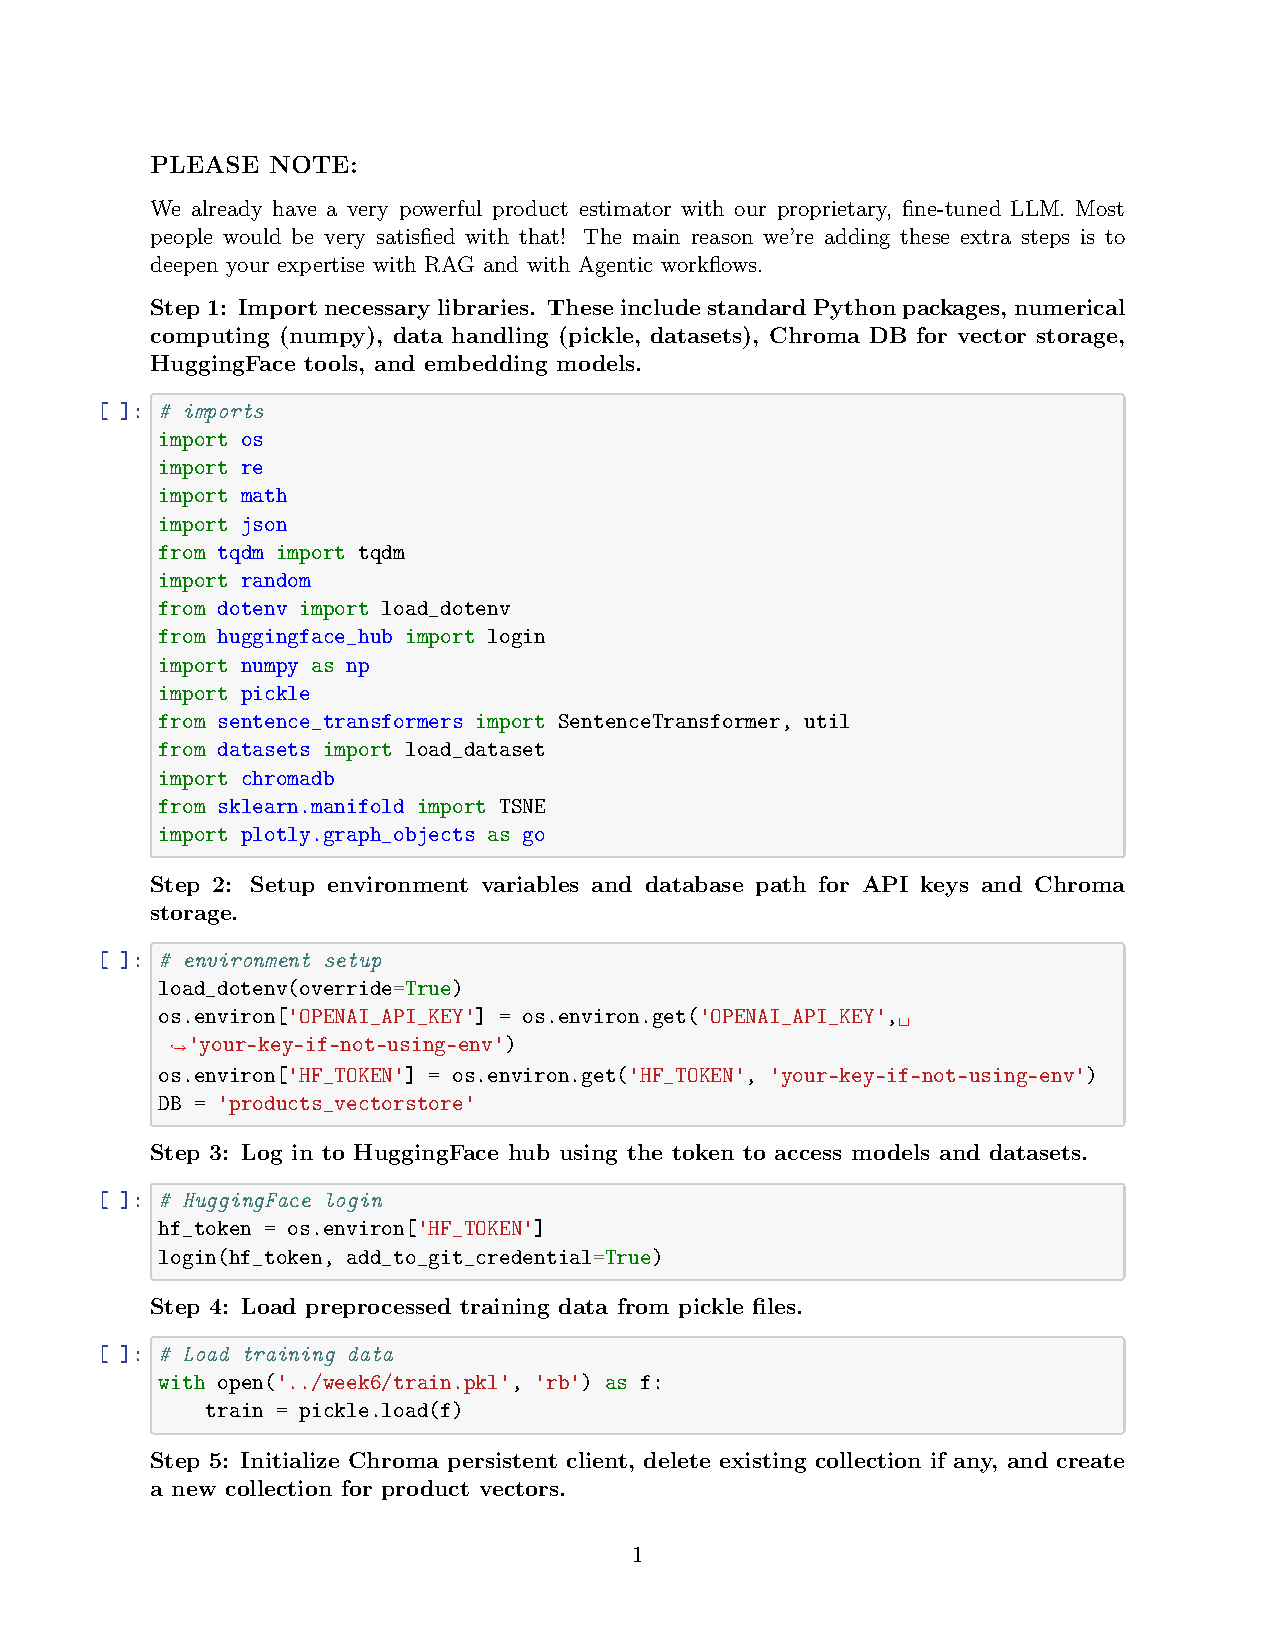
\includepdf[pages=-]{DAY2.pdf}



\section{Hallmarks of an Agentic AI Solution}
\begin{tcolorbox}[title={1. Decomposition of Larger Problems into Smaller Steps}, colback=blue!5!white, colframe=blue!75!black]
An \textbf{Agentic AI system} decomposes complex problems into smaller, manageable steps. Each step is handled by an \textit{independent agent} or \textit{specialized process}, allowing for:  
\begin{itemize}
    \item \textbf{Parallel processing} for faster execution.
    \item \textbf{Error reduction} by isolating tasks.
    \item \textbf{Task modularity} to reuse and recombine solutions.
    \item \textit{Scalable problem solving} for multi-domain challenges.
\end{itemize}
This approach ensures that large goals can be achieved efficiently without overwhelming any single component.
\end{tcolorbox}
\vspace{0.5cm}
\begin{tcolorbox}[title={2. Use of Tools, Function Calling, and Structured Outputs}, colback=green!5!white, colframe=green!75!black]
Agents can call \textit{external tools}, \textit{APIs}, or defined functions to extend their capabilities. Structured outputs ensure clear and reliable results. Key benefits include:  
\begin{itemize}
    \item \textbf{Precision:} Outputs like JSON or tables can be directly processed.
    \item \textbf{Reliability:} Reduces ambiguity in multi-agent workflows.
    \item \textbf{Interoperability:} Allows agents to communicate results seamlessly.
    \item \textit{Error handling:} Structured formats make it easier to validate and parse responses.
\end{itemize}
\end{tcolorbox}
\vspace{0.5cm}

\begin{tcolorbox}[title={3. Collaborative Agent Environment}, colback=orange!5!white, colframe=orange!75!black]
Agents operate in a shared environment enabling \textbf{collaboration and coordination}:  
\begin{itemize}
    \item \textbf{Specialized knowledge:} Different agents contribute unique skills.
    \item \textbf{Task distribution:} Efficient division of labor for complex goals.
    \item \textit{Real-time communication:} Agents exchange updates to optimize outcomes.
    \item \textit{Conflict resolution:} Conflicting suggestions can be reconciled by higher-level agents.
\end{itemize}
Collaboration enhances overall system performance beyond the capability of any single agent.
\end{tcolorbox}
\vspace{0.5cm}

\begin{tcolorbox}[title={4. Planning and Coordination Agent}, colback=red!5!white, colframe=red!75!black]
A \textbf{planning agent} orchestrates activities across all agents:  
\begin{itemize}
    \item Determines the sequence of tasks based on dependencies.
    \item Dynamically adjusts plans according to intermediate results.
    \item Prioritizes critical steps to achieve goals efficiently.
    \item Monitors progress and reallocates resources as needed.
\end{itemize}
This ensures that complex workflows are executed coherently and reliably.
\end{tcolorbox}
\vspace{0.5cm}

\begin{tcolorbox}[title={5. Autonomy and Persistent Memory}, colback=purple!5!white, colframe=purple!75!black]
Agentic AI demonstrates \textbf{autonomy} and maintains \textit{persistent memory}, which allows:  
\begin{itemize}
    \item \textbf{Independent operation} without constant human intervention.
    \item \textbf{Learning from past interactions} to improve decision-making.
    \item Retention of critical information across sessions for long-term planning.
    \item \textit{Cumulative knowledge growth}, enabling adaptation to new situations.
    \item Capability to handle multi-step and long-horizon tasks effectively.
\end{itemize}
\end{tcolorbox}
\vspace{1cm}
\includegraphics[width=1\textwidth]{hallmark.png}
